
\documentclass{article}

%\usepackage[swedish]{babel} % Försvenskar autoinput ex. "Del 1" ist. för "Part 1"

% Tables
\usepackage{siunitx}	% Simple units and decimal point alignment in tables
\usepackage{booktabs}	% Pretty booktabs
\usepackage{multirow}	% Multi- rows and columns + cell-specific positioning
\usepackage{multicol}	% Primarily for setting text into columns
\usepackage{rotating}	% Rotated tables
\usepackage{pgfplotstable}	% Import excel tables from .csv files
\usepackage{longtable}	% Multi-page spanning tables

% Packages
\usepackage[utf8]{inputenc}	% Tillåter å ä ö som direkt input
\usepackage{graphicx}	% Figures
\usepackage{subcaption}	% Subfigures
\usepackage{amsmath}	% Alignment of equations
\usepackage{lipsum} 	% Lorem Ipsum
\usepackage{setspace}	% Switch between simple- and double spacing
\usepackage{framed}		% Environment that frames everything in it
\usepackage{hyperref}	% Hyperlinks, websites, e-mail
\usepackage{enumitem}	% Spika bullet symbols för \itemize och stil för \enumerate
\usepackage{listings}	% Miljö för att formatera kod. Språkspecifik.
\usepackage[T1]{fontenc}	% Tillåter tolkning av å ä ö m.m.
\usepackage[a4paper,textwidth=500pt,textheight=700pt]{geometry}	% Spikar marginaler
\usepackage{float}	% Allows more advanced positioning of floats
\usepackage[parfill]{parskip}	% Uses spacing instead of indents on line breaks

\usepackage[format=plain,
            labelfont=it,
            textfont=it]{caption}

\begin{document}
    \pagenumbering{gobble}
	\begin{figure}
		
\includegraphics[width=0.3\linewidth]{images/kth_logga.png}
	\end{figure}
	\title{\vspace{10mm} Saturation Mutagenesis of the Z-domain\\{\Large Degree project, in Biotechnology, first level}}
	\author{Karin Alexandersson Ros, Richard Brunsell, Matilda Fresk,\\Alfred Kedhammar, Gabriella Rossi \\ \\ Supervisor \\ John Löfblom}
	\maketitle

	\newpage
	\section*{Sammanfattning}
		Målet med projektet är att förbättra affiniteten mellan Immunoglobulin G (IgG) och den bindande Z-domänen hos Protein A från stafylokocker genom att skapa ett bibliotek med muterade oligonukleotider. Z-domänen används inom bioteknik för många applikationer som skulle dra nytta av en ökad affinitet. 
		
		För att påverka affiniteten genomfördes en mättnadsmutagenes där aminosyror blir substituerade för alla andra aminosyror. Alla ytexponerade aminosyror substituerades samt ytterligare några av instresse. Mättnadsbiblioteket bestående av 912 olika linjära enkelsträngade oligonukleotider, där alla har en punktmutation, erhölls via en tredje part. Plasmiderna extraherades från \textit{Escherichia coli} för att kunna ersätta nonsenssekvensen i plasmiden med en funktionell Z-domän. Innan ersättningen gjordes hade både plasmiden och den funktionella Z-domänen amplifierats via polymerase chain reaction (PCR). Plasmiderna sattes samman och transformerades in i \textit{E.coli} för att odla upp produkt. Efter amplifiering i \textit{E.coli} extraherades plasmiderna, renades och slutligen transformerades in i \textit{Staphylococcus carnosus} för ytterligare amplifiering. Z-domänen uttrycks på ytan hos \textit{S.carnosus}. För att analysera resultaten genomfördes flödescytometri och cellsortering.
		
		Affiniteten mellan IgG och Z-domänen är relativt högt i vildtypen, 20 nM \cite{john}, men genom mättnadsmutagenesen kommer affiniteten påverkas och förhoppningsvis förbättras. Resultaten som erhölls från mättnadsmutagenesen gav varianter med både förbättrad och försämrad affinitet. Projektet har potential att identifiera punktmutationer och ge användbar information för framtida design av mättnasbibliotek.
	
	\newpage
	\section*{Abstract}
		The project aims to enhance the affinity between the Immunoglobulin G (IgG) and the binding Z-domain from staphylococcal Protein A by creating a library with mutated oligonucleotides. The Z-domain is commonly used in biotechnology for many applications that would benefit from a high affinity. 
		
		To affect the affinity a saturation mutagenesis was performed where amino acids were substituted for all other amino acids. All surface-exposed residues were substituted and additionally several others of interest. The site saturation library consisting of 912 different plasmids, each with a single point mutation, was obtained via a third party. The plasmids were extracted from \textit{Escherichia coli} in order to replace the non-functional dummy sequence in the plasmid with a functional Z-domain after having amplified both the plasmid and the insert with polymerase chain reaction (PCR). The plasmids where assembled and then transferred to \textit{E.coli} to grow a lot of product, after having been amplified in \textit{E.coli} the plasmids where extracted and purified to be able to transfer them into \textit{Staphylococcus carnosus} for further amplification. The Z-domain is expressed on the surface of \textit{S.carnosus}. Flow cytometry and cell sorting was performed to analyze the results. 
		
		The affinity between IgG and the Z-domain is relatively high in wild type, 20nM \cite{john}, but through the performed mutations the affinity will be affected and hopefully it has increased. The results obtained from the saturation mutagenesis contained variants with both higher and lower affinity. The project has the potential to identify single-point mutations and give useful information for future designing of saturation libraries. 
	
	\newpage
	\tableofcontents
	
	\newpage
	\pagenumbering{arabic}
	\begin{multicols}{2}
	\section{Background}
	\subsection[Libraries and directed evolution]{Libraries and directed\\evolution}
	Earlier methods of producing protein-based affinity reagents \textit{in vivo}, involves injecting pathogens into the bloodstream of a laboratory animal, and then rely on the immune system and B-cells of the animal, to produce the antibodies. The blood is later drawn from the animal to collect the desired antibody with affinity for the injected pathogen. 
	
	In vitro-based methods, such as directed evolution, phage display and library technology have been developed as an alternative to immunization of laboratory animals for \textit{in vivo} protein-based lab experiments and screening for affinity reagents such as antibodies. The method \textit{directed evolution} won the Nobel Prize in Chemistry 2018 \cite{noauthor_nobel_nodate}.

	The above mentioned in \textit{vitro methods} are based on altering a desired protein sequence by varying base pairs coding for the amino acids in a DNA-sequence. The desired protein without the modifications, is referred to as the wild type. The result is a library containing of millions or billions improved or worse versions of the wild type protein. This library is used to screen for the versions with the highest affinity for the specific pathogen. Thus, this method meets the same end goal of producing protein-based affinity reagents as the traditional method, but without the need for laboratory animals.
	
	\subsection{Affinity maturation}
	Affinity maturation is the engineering process of improving an already existing affinity protein to obtain an even higher affinity. One approach to obtain this is to use an error-prone PCR to consciously introduce changes in the original DNA sequence to create a variation of different versions of the original protein \cite{mishra_insights_2018}. The result of error prone PCR is often low quality libraries compared to site directed alternatives with a majority of non functional protein. The non functional proteins are a result of induced new diversity in parts of the protein disconnected from the paratope and subsequently introduced deletions \cite{mccullum_random_2010}. The folding of the protein is crucial and small changes in the amino acid structure can result in cardinal changes in the functionality of the protein. 
	
	%\vfill\null
	%\columnbreak
	
	\subsection[Saturation mutagenesis, site directed mutagenesis and alanine scan]{Saturation mutagenesis, site\\directed mutagenesis and\\alanine scan}
	To analyze the function of an amino acid in relation to a whole protein site directed mutagenesis is often performed by doing an alanine scan. In an alanine scan a single surface-exposed residue in the paratope is substituted for alanine and the effect this has on the protein is analyzed \cite{morrison_combinatorial_2001}.
	
	A similar method that provides a more thorough analysis is site saturation mutagenesis which is when all surface-exposed residues are substituted for all of the different amino acids. This method provides a collection of mutagenesis products that all have a different amino acid in the target position, making the library so called saturated. 
	
	When producing a library through mutagenesis it is important to consider the desired randomness whilst being able to eliminate the parental DNA. When performing mutagenesis, most methods use an annealing primer, commonly performed by synthesizing it as a mixture of oligonucleotides that are identical to the parental DNA, only having a specific positions being non-identical. By creating a primer that is identical, allows the primer to anneal to the parental DNA whilst the non-identical positions creates the diversity of the product \cite{siloto_site_2012}. 
	
	Site maturation mutagenesis is a simple and effective way for creating variants of proteins that would have taken a long time to occur naturally, or if even at all. 
	 
	
	\subsection{Immunoglobulin G}
	Immunoglobulin G is the most common antibody found in vertebrates consisting of two identical light chains and two identical heavy chains that are connected by disulfide bonds. An IgG antibody consists of two fragments, the antigen binding region (Fab) and the crystallizable region (Fc), where the Fab region contains the paratope which has the surface-exposed residues. The IgG antibody works to create a connection between the antigen and the body’s effector system, the fab region binds to the antigen and the Fc region is connected to the effector system \cite{sanders_chapter_2008}. 
	
	\subsection{The Z-domain}
	There have been several bacterial immunoglobulin (Ig)-receptors found in later years, with Staphylococcal Protein A (SpA) being well studied, and they have come to be important for the binding, identification and purification of immunoglobulins. Protein A was the first described bacterial immunoglobulin receptor and is found in the cell wall of \textit{Staphylococcus aureus}, it has a molecular weight of 42 kDa and binds to the Fc region of IgG. By studying the structural changes that occurs when SpA binds to the Fc regions shows that this interaction involves the Z domain of SpA, studies have also shown that SpA can interact with the Fab region \cite{justiz-vaillant_bacterial_nodate}. 
	
	The SpA has become the foremost used reagent in immunological methods and a variety of applications have been developed. All methods that use SpA is based on the selective binding between the SpA and the Fc region of the IgG, these methods are divided into two categories. The first category involves methods that use purified SpA that have been labeled with a tracer group in order to detect and quantify antibodies and antigens. The second category uses immobilized SpA either as a part of the cell membrane of the bacteria or with purified SpA covalently bound to a solid support in order to isolate whole IgG or subclasses, to divide cells, selectively absorb IgG or to precipitate antibody-antigen complexes \cite{langone_applications_1982}.
	
	\subsection{Polymerase chain reaction, PCR}
	Amplification with PCR is a common and effective method to generate a large number of copies of a desired DNA fragment. It is widely used because of its simplicity and ability to create product fast. The most prominent disadvantage with PCR amplification has to do with the primers needed. Since primers are necessary for this method, the sequence of the target region has to be known \cite{li_chapter_2008}. 
	
	\subsection{\textit{In vitro} assembly}
	In vitro assembly is a method for constructing a complete circular plamsid. This method uses exonucleases that continously remove nucleotides at the 5’ ends of the fragments, leaving single stranded DNA regions. With the overlap created by the placement of the PCR primers, the ends of the plasmid and insert fragments can anneal, creating a complete plasmid. The regions where the exonuclease proceeded too far and left ssDNA outside the overlap is extended via DNA polymerase, and the nicks are sealed with cellular ligase \textit{in vivo} or \textit{in vitro} \cite{john}.
	
	\subsection{Flow cytometry and cell sorting}
	Flow cytometry is a technique used in analysis of cells and together with the cell sorting technique it is a powerful and efficient tool used in laboratory work with prokaryotic and eukaryotic cells \textit{in vitro}. The method uses a combination of fluidics, optics and electronics to generate diagrams and mechanically sort viable cells one by one in different vials according to characteristics. The information obtained by this technique include measurement in size, cell count, cell cycle and characteristics. It is possible to obtain specific information on individual cells \cite{flow}.
	
	Cell sorting is then generated based on the information obtained by selecting gates in the plot diagram. Gates are marked areas in the plot diagram that is selected by the researcher for sorting. The flow cytometry is run once again and the computer will then sort out the cells that are gated in different tubes using electric fields. In this lab we are interested in sorting out two types of cells. One gate with high affinity between Fc region and Protein A and another gate corresponding to lost affinity. The sorted cells can furthermore be sequenced to collect information on which mutations give higher affinity, and which mutations result in lower affinity.
	
	When working with fluorophores, it is important not to subject them to light causing them to fade, which would make it hard to see any results, it is also important for this method that the fluorophore has bound to the antibody. Whilst wanting to avoid having no signal it is not desired to have an excess fluorescent signal either. To distinguish between different affinities, the Z-domains on the cells must compete for the fluorophores with the better binding mutants binding more fluorophores. A too high concentration would saturate all the mutants and no difference could be seen in affinity.
	
	
	\subsection{Overview of the procedure}
	The procedure will comprise affinity maturation of the IgG-binding Z-domain from Staphylococcal Protein A. To create an enhanced affinity within the Z-domain, a saturation mutagenesis will be conducted.
	
	In this project inspiration is taken from the alanine scan but instead of investigating substitution to alanine exclusively, substitution of every amino acid will be tested. This will give a broader spectrum of variety of combinations of the protein and the possibility to find a higher affinity, when alanine scan only provides information of silencing one position at the time.
	
	Saturation mutagenesis will be conducted in which mutants of selected amino acids are mutated by replacing them with all different amino acids to see the influence on the affinity. By doing this, results from all possible substitutions, not just alanine, will be collected. This project will be limited to individual point mutations in order to examine the impact of specific mutations on the protein. Once the effects of the mutations have been observed in a flow cytometer, the data will be analyzed. The individual point mutations will give 912 different variants of the Z domain and when the effect of the individual mutations has been studied they can be combined to create an even more targeted library \cite{john}.
	
	\section{Aims of the project}
	The aim of this project at large is to generate, interpret and present data regarding how all possible point substitutions of 19 amino acids in the Z-domain affect it’s affinity for the human antibody immunoglobulin G domain fragment crystallizable to facilitate the development of a targeted library for further affinity maturation.
	
	In further detail, this aim amounts to a primary goal of producing a library consisting of 912 mutated variants of the Z-domain (19 substitutions on 48  sites respectively), each coding for a unique Z-domain. The next interim is to assemble an aliquota of this library to a suitable vector allowing for selective growth and surface expression on a bacterial cell. The vector is then transformed into competent cells to form the in-vivo library, which can be amplified or stored on demand. The affinity of the library can then be analyzed and compared to the wild type using fluorescence activated cell sorting (FACS), the results of which can be traced back to it’s originating substitution using DNA-sequencing.
	
	\section{Project plan \\ and methodology}
	\subsection{Library construction}
	\label{met_lib_cons}
	The complete library consisted of 912 different DNA oligonucleotides, each with a single point mutation (see appendix \ref{lib_seq}).
	
	The mutation was at one of the 48 predetermined positions of the Z-domain of Protein A, chosen so that the mutation affects the surface of the protein and thus potentially the relative binding to IgG Fc. The point mutations were substitutions of the original amino acid to any of the other 19 amino acids not present in the wild-type variant of Protein A’s Z-domain.
	
	Oligonucleotides of the mutated Z-domain were produced and sequence verified via a third party, Twist Bioscience (see appendix C). The specified library order arrived in a 96-well plate. There were 48 wells, one for each altered position and each containing 19 variants of amino acid substitutions in that position. 
	
	The wells each contained approximately 50 ng of dry freeze material, these were diluted in 100 $\mu$L MQ to an approximate concentration of 0.5 ng/$\mu$L.
	

	\subsection{Library vector}
	The plasmid pSCZ1 \cite{fleetwood_simultaneous_2015} was used as a vector for the library. This plasmid contains the necessary expression sequences such as ORI, antibiotic resistance genes, and the surface expression and detection protein coding sequences. However, pSCZ1 does not contain a functional Z-domain but a dummy sequence in place. The dummy sequence is filled with nonsense and stop codons in different reading frames to ensure it does not interfere with any desired plasmid, should it be expressed. See appendix \ref{primer_seq}. 
	
	These plasmids were extracted and purified from RR1 \textit{E.coli} using a QIAquick Plasmid Purification Kit (QIAGEN). A gel electrophoresis was performed to ensure that the purification was successful.
	
	\subsection{Amplification of plasmid and insert via PCR}
	The plasmid pSCZ1 and the insert library were amplified by Polymerase Chain Reaction (PCR), according to PCR Protocol for Phusion \textregistered High-Fidelity DNA Polymerase (M0530) at 50 $\mu$L (New England Biolabs). The 49 reactions (48 variants + negative control) performed on the insert library used HF buffer and the 8 reactions (7 parallel reactions + negative control) performed on pSCZ1 used GC buffer.
	
	The PCR protocol for both procedures was derived using the NEB Tm calculator.
	A gel electrophoresis was performed to verify product. 
	
	Primers for both amplicons were designed using $Benchling^{TM}$ to fit the recommendations of above-mentioned protocol and synthesized by Integrated DNA Technologies, BVBA. The insert primers were designed so that the Z-domain and an overhang of ~200bp were included. The vector primers excluded the innate nonfunctional dummy sequence, and had a similar overlap of ~200bp. See appendix \ref{primer_seq}.
	
	The PCR-product was verified using gel electrophoresis.
	Original plasmid template in the pSCZ1 PCR product was destroyed using DPNI. All insert reactions and vector reactions were pooled and purified using QIAquick PCR Purification Kit (QIAGEN). 
	
	The purification was verified using gel electrophoresis.
	
	 
	\subsection{Assembly}
	The PCR amplification of the vector created a linear construct. This fragment and the insert had an homologous region of ~200bp at each end. \textit{In vitro} assembly was used to assemble the linear constructs into a complete, circular, plasmid. 
	
	The assembly was carried out using two different kits, NEBuilder HiFi DNA Assembly Kit, and In-Fusion HD Cloning Kit. In the NEBuilder Kit, 100 ng of vector and 5.76 ng of insert were added to NEBuilder HiFi DNA Assembly Master Mix to give a ratio of vector to insert of 1:3.
	
	The amount of NEBuilder HiFi DNA Assembly Master Mix added to the cells for the transformation was varied at 2, 3 and 5 $\mu$L respectively to evaluate which was the most efficient method. For the In-Fusion HD Cloning Kit the volume was kept constant at 2.5 .
	
	In the In-Fusion Kit assembly, 100 ng of vector and 14.65 ng of insert were added to 5X In-Fusion HD Enzyme Premix to a ratio of vector to insert of 1:5. These mixtures were incubated at 50$^o$C for 15 minutes after which they were transformed to \textit{E.coli}.
	
	The transformation to \textit{E.coli} was performed according to respective kit protocols, however the following deviations were made. The In-Fusion protocol calls for a washing step which was omitted. All the reaction mixture from both kits were used and spread on plates. 
	
	As an initial trial of the different kits, each kit was used in triplicate, with one negative control.
	
	\subsection{Amplification in \textit{E.coli}}
	The assembled plasmids were transformed to\textit{E.coli} via heat shock at 48$^o$C and grown on ampicillin plates overnight at 37$^o$C. The assembled plasmid contains the gene for beta-lactamase to ensure selective growth.
	
	The number of colonies were counted and used to calculate library coverage using summarized probability and a negative exponential distribution formula.
	
	The plasmids were harvested from the \textit{E.coli} cultivation with a QIAquick Maxi Plasmid Purification Kit (QIAGEN).
	
	\subsection{Transformation and amplification in \textit{S.carnosus}}
	The amplified and purified vectors from the \textit{E.coli} cultivation were transformed into electrocompetent \textit{S.carnosus} using electroporation.
	
	The plasmid solution and 240 $\mu$L electrocompetent cells were thawed on ice for 5 min. The cells were then incubated at room temperature (RT) for 30 min, mixed and centrifuged down. The cells were then heat-shocked in a water-filled heat block at 56$^o$C for precisely 1 min 30 seconds, after which 1 mL 0.5 M sucrose + 10\% glycerol were immediately added to the tube which was then mixed by inversion.
	
	The tube was then centrifuged at 4500x g (7000 RPM) for 10 min at RT. The supernatant was discarded. After this, 140 $\mu$L 0.5 M sucrose + 10\% glycerol was added and the sample was mixed by pipette. Subsequently, 4 $\mu$L plasmid was added using a 10 $\mu$L filtered pipette tip, the tube was then mixed by pipette and centrifuged down. The tube was incubated at RT for 10 minutes.
	
	A BioRad MicroPulser was used for the electroporation with voltage 2.3 kV and time constant 1.1 ms.
	
	The contents of the tube were evenly divided between 4 parallel electroporations, as follows. From the cell suspension, 55 $\mu$L were added to a cuvette using a pipette and a 100 $\mu$L filter tip. The cuvette was then tapped into the bench to get rid of air bubbles. To the cuvette, 1 mL of B2 medium was added and the electroporation was performed. Immediately after, an additional 400 $\mu$L B2  medium was added, the sample was then mixed by pipette and transferred to an eppendorf tube.
	
	The cells were then incubated at 37$^o$C under rotation for 2 hours after which 200 $\mu$L from each suspension was plated on RT-incubated growth plates with 10 ug/mL chloramphenicol at 37$^o$C for 24 hours. The cells were then incubated at RT for an additional 3 days.
	
	The colonies on the plates were counted and library coverage was calculated again.
	
	For amplification, the cells on the plates were transferred to a solution of Tryptic Soy Broth with yeast extract (TSB+Y) and chloramphenicol and grown at 37$^o$C for 24 hours.

    \newpage
    
	\subsection{Flow cytometry and cell sorting}
	\end{multicols}
	\begin{figure}[H]
		\centering
		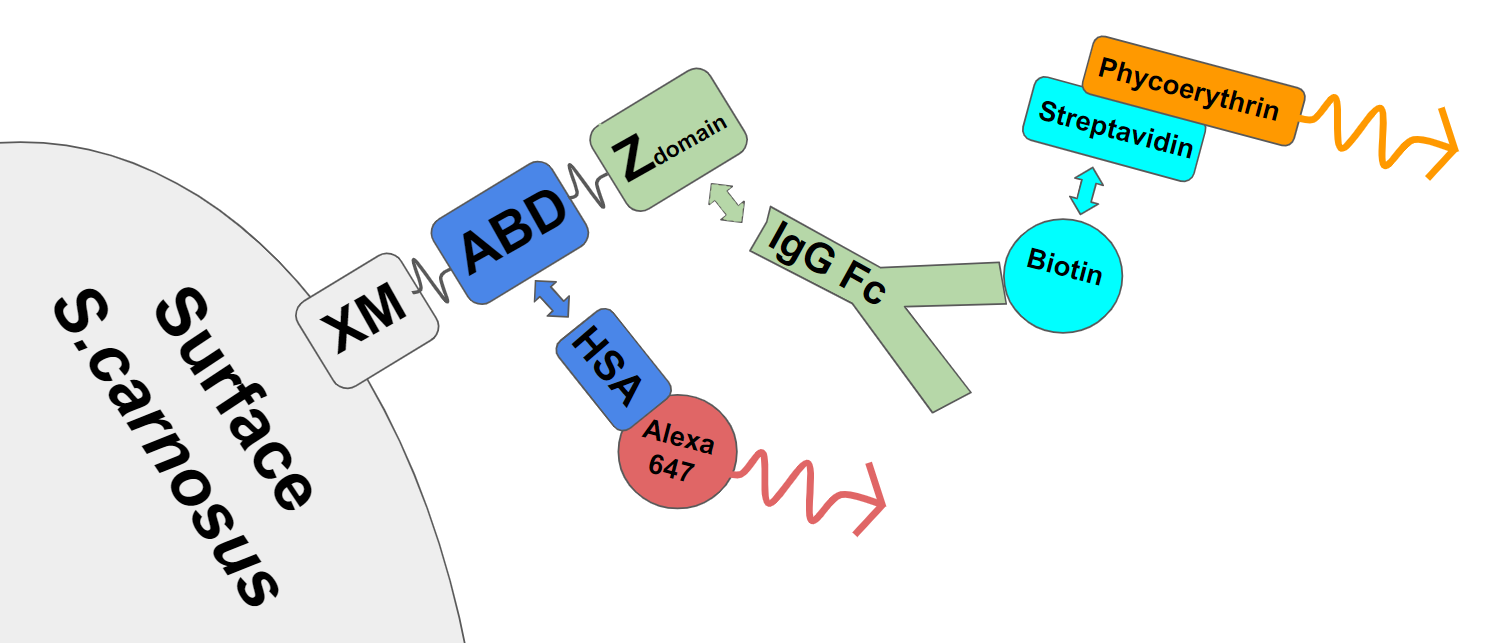
\includegraphics[width=\linewidth]{images/surface.png}
		\caption{Schematic representation of the fluorophores present on the surface of \textit{S.carnosus} prior to flow cytometry.}
		\label{surface}
	\end{figure}
	\begin{multicols}{2}
	 	
	 In this lab, the Z-domain is expressed on the outer membrane of the
 	\textit{S. carnosus}. To examine the affinity for the mutated Z-domain, two fluorophore-linked groups with different wavelengths were used and incubated with the cells for the flow cytometry and cell sorting, see figure \ref{surface}.
	
	Since the mutations were specifically induced by saturation mutagenesis instead of a non specific method such as error prone PCR, it is possible to know which part of the protein is constant between the mutants. The HSA bound the albumin binding domain (ABD), this antibody measurement was used to count the amount of Protein A on each cell. The second antibody bound to the mutated region of the protein, testing the affinity for that specific mutant. In combination of the two, information on the relative amount of Protein A on each cell together with the amount of antibody binding to the mutated region, the affinity between the mutated Protein A and Fc region on IgG was measured \cite{john}. This information generated a plot diagram with one fluorescence on the x-axes and the other fluorescence on the y-axes.
	
	A flow cytometry was performed on the library and the wild-type protein to determine the optimal concentration of IgG. From overnight cultures 15 $\mu$L cells were washed with 800 $\mu$L phosphate buffered saline with 0.1\% Pluronic (PBSP). The cells were centrifuged at 6000 RPM in 4$^o$C for 6 min and the supernatant was discarded. The resulting cell pellets were resuspended in 250 $\mu$L PBSP containing 0.4, 1, 4, 20 and 100 nM biotinylated IgG. The cells were incubated at RT under gentle mixing for 45 minutes. The cells were washed with 180 $\mu$L ice-cold PBSP, and resuspended in 230 $\mu$L ice-cold PBSP containing the fluorophores HSA-Alexa-647 conjugate and Streptavidin Phycoerythrin-conjugate (SAPE) at a 1:500 dilution. The cells were then incubated on ice and in the dark for 45 min, after which they were washed with 180 $\mu$L ice-cold PBSP and resuspended in 300 $\mu$L ice-cold PBSP in flow cytometer tubes. The ratio of emission for the used florophores 580 and 665 nm was measured.
	
	For cell sorting, the procedure above was repeated using a FACS machine with IgG concentrations 0.4 and 10 nM. The cells with higher affinity for IgG than the majority of binding cells were sorted at IgG concentrations of 0.4 and 10 nM. The cells with average binding affinity to IgG were sorted at IgG concentrations of 10 nM. The non-binding cells were sorted at IgG concentration 10 nm. The affinity gates were combined with a gate comparing front- and backscatter to only sort cells with a profile similar to \textit{Staphylococcus}. The cells from the gates were grown on separate plates with chloramphenicol in 37$^o$C overnight. 

	\subsection{Sequence analysis}
	From each plate 96 colonies were individually picked and amplified with PCR. To verify that the PCR was successful 10 colonies from each PCR plate were picked and analysed with gel electrophoresis. The amplified colonies were sent to Microsynth Seqlab Sequencing for bi-directional sequencing with primers SAPA-23 and SAPA-24 (see appendix \ref{primer_seq}).
	
	The returned sequencing results were obtained in the form of .fasta and .ab1 files for each primer. The .fasta files were converted to .csv using console commands. Next, a Matlab script was constructed (see appendix \ref{script}). The script compiled all SAPA-23 sequencing results to a data vector, then it used sequences 20 bp up- and downstream of the substituted section of the Z-domain to align them in the correct reading frame. Next it used open-source software to translate the aligned nt sequences to their corresponding aa sequences. It then compared these sequences to the aa sequence of the wild type Z-domain and subsequently found the positions where AA substitution had taken place and in what qualitative form. During this process, the script also continuously classified and documented different discrepancies in the sequencing results that would prevent them from generating the desired results.
	

	\section{Results}
	\subsection{Library construction}
	The library was delivered as specified in section \ref{met_lib_cons}.
	
	\subsection{Library vector}
	The successful extraction and purification of pSCZ1 from RR1 \textit{E.coli} was verified with gel electrophoresis, see figure \ref{pscz1_renad_fr_ecoli}. The ladder to the left is used to verify the length of the purified fragment. Since the ladder contains a known composition of fragments with known lengths, it is possible to verify the successful extraction.
	
	\begin{figure}[H]
		\centering
		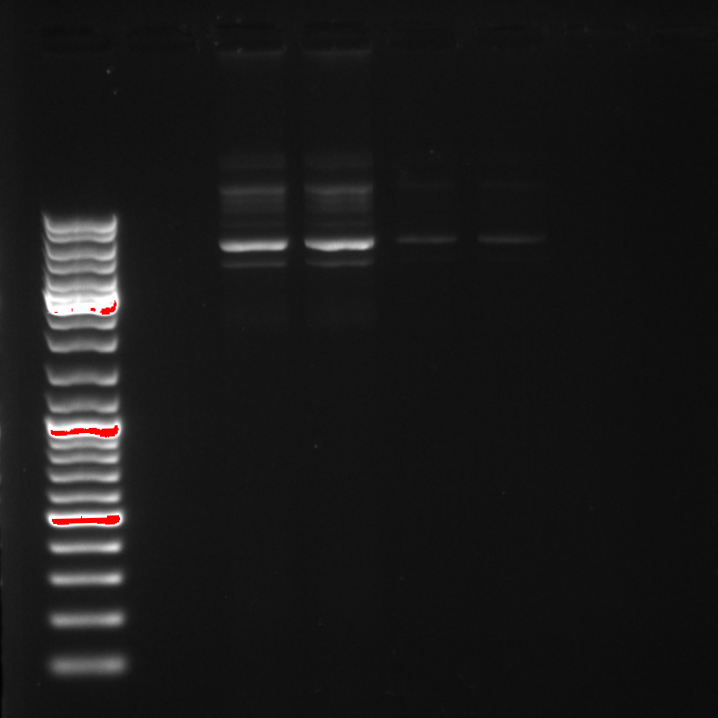
\includegraphics[width=0.7\linewidth]{images/pscz1_renad_fr_ecoli.png}
		\caption{Gel verifying the extraction of pSCZ1 from RR1 \textit{E.coli}.}
		\label{pscz1_renad_fr_ecoli}
	\end{figure}
	
	\vfill\null
	\columnbreak
	
	\subsection{Amplification of plasmid and \\insert}
	After the plasmid, pSCZ1, had been extracted a PCR was performed to amplify both the plasmid and the delivered inserts to create many copies. The PCR-product was verified using gel electrophoresis, see figure \ref{ampl}.
	
	\begin{figure}[H]
		\centering
		\begin{subfigure}{0.7\linewidth}
			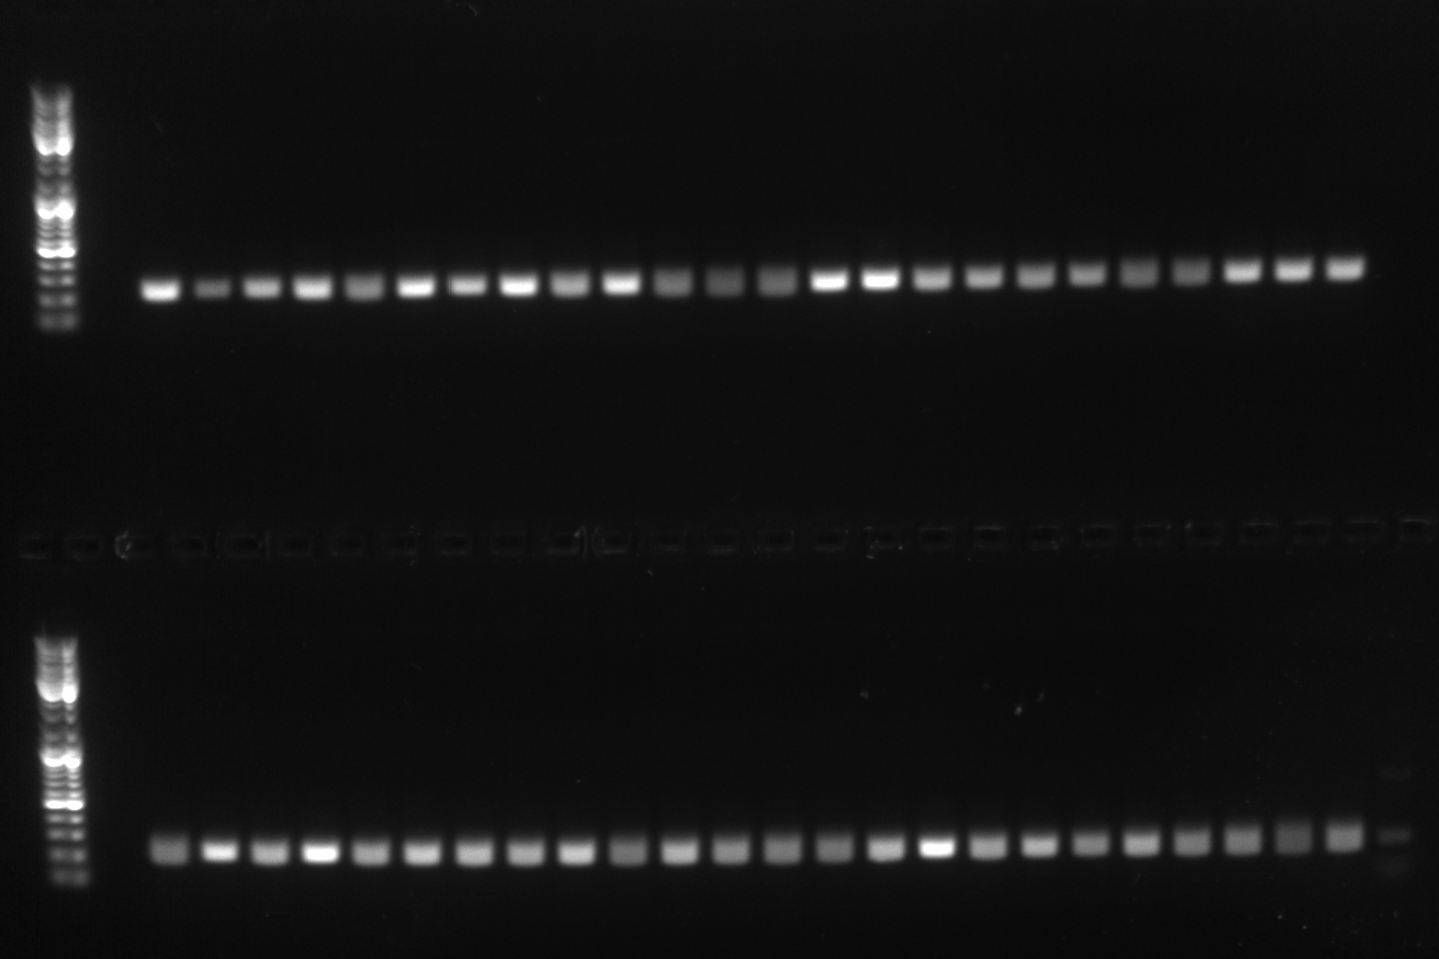
\includegraphics[width=\linewidth]{images/oligos_efter_PCR.png}
			\caption{Library amplicon.}
		\end{subfigure}
		
		\begin{subfigure}{0.7\linewidth}
			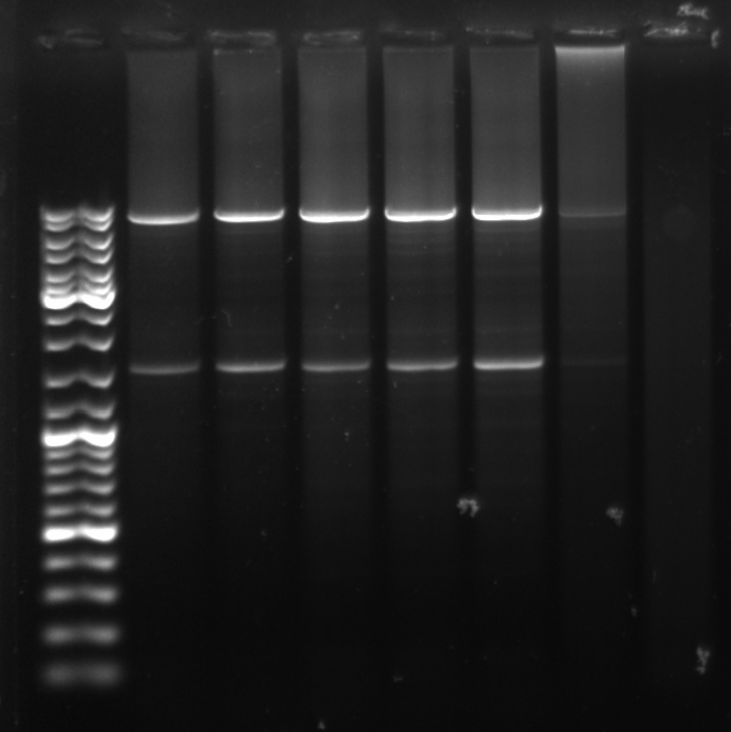
\includegraphics[width=\linewidth]{images/pscz1_efter_PCR.png}
			\caption{Plasmid amplicon.}
		\end{subfigure}
		\caption{Gels verifying successful PCR-amplification.}
		\label{ampl}
	\end{figure}
	
	\vfill\null
	\columnbreak
	
	The subsequent purification was verified using gel electrophoresis, see figure \ref{rening}.
	
	\begin{figure}[H]
		\centering
		\begin{subfigure}{0.7\linewidth}
			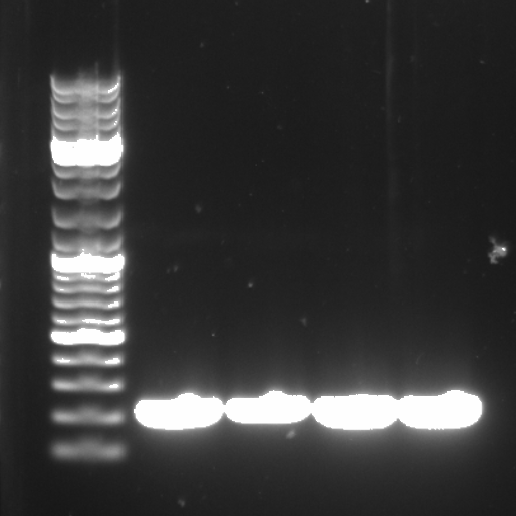
\includegraphics[width=\linewidth]{images/oligos_efter_PCR_renad.png}
			\caption{Library purification.}
		\end{subfigure}
		
		\begin{subfigure}{0.7\linewidth}
			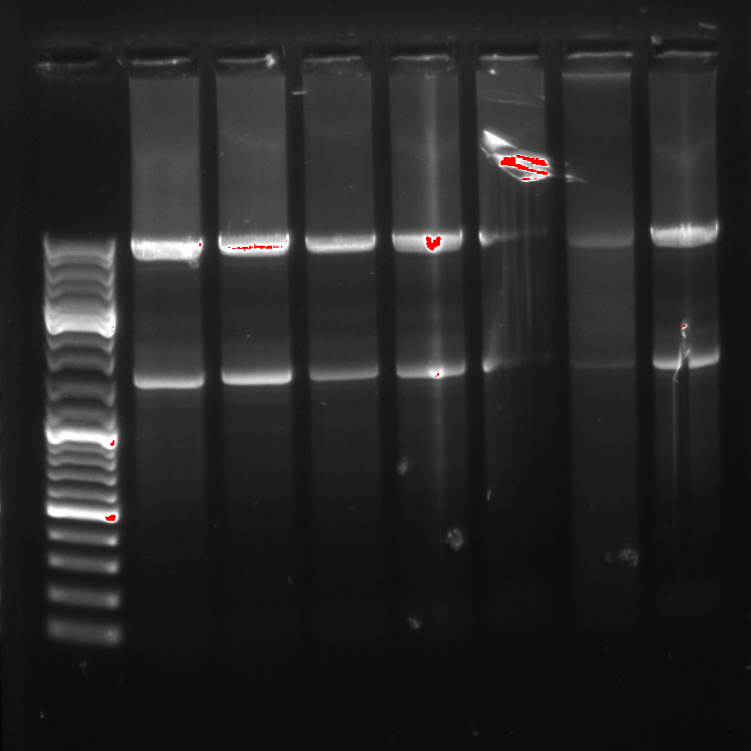
\includegraphics[width=\linewidth]{images/pscz1_efter_PCR_renad.png}
			\caption{Plasmid purification.}
			\label{pscz1_efter_PCR_renad}
		\end{subfigure}
		\caption{Gels verifying successful purification.}
		\label{rening}
	\end{figure}

	\subsection{Assembly}
	The concentrations of the plasmid and the inserts were determined with nanodrop (see appendix D). As the gel electrophoresis of the plasmid displayed a potential incomplete product in addition to the expected product, two thirds of the measured concentration was assumed to be the complete plasmid product, while the incomplete sample was ignored as it would not have the overlapping regions to proceed through assembly.
	
	\begin{table}[H]
		\begin{center}
			\caption{Concentrations obtained via nanodrop. Sample 6 is omitted from the mean, and corresponds to well 6 in figure \ref{pscz1_efter_PCR_renad}}
			\label{nanodrop_tab}
			
			\begin{tabular}{c|c|c|c|c|c|c}
				\toprule
				\multicolumn{7}{c}{\textbf{Concentration ng/$\mu$L}} \\
				\midrule
				89.2 & 85.3 & 73.9 & 79.3 & 78.9 & 44.5 & 73.9 \\
				\bottomrule
				\multicolumn{1}{c}{\textbf{Mean}} & \multicolumn{5}{c}{} & \textbf{80.1} \\
			\end{tabular}
		\end{center}
	\end{table}

	A preliminary transformation of the assembled plasmid was performed, and after an overnight cultivation the NEBuilder kit was determined to be of interest for continued projects as the number of colonies was tenfold compared to the In-Fusion kit. The remaining of the purified fragments were assembled the following day. The NEBuilder reaction mixture was performed in quintuplicate of the three different concentrations yielding a total of 15 growth plates, while the In-Fusion mixture was plated on 3 growth plates.
	
	\setlength{\tabcolsep}{4pt}
	\begin{table}[H]
		\begin{center}
			\caption{Table of colony count on respective growth plate from different assemblies}	
			\begin{tabular}{c|c c c|c|c}
				\toprule
				\textbf{Kit} & \multicolumn{3}{c|}{\textbf{Colony count}} & \textbf{Avg.} & \textbf{Neg. control} \\
				\midrule
				In-Fusion & 199 & 168 & 196 & 187.6 & 1 \\
				NEBuilder & 1088 & 1136 & 971 & 1065 & 22 \\
				\bottomrule
			\end{tabular}
		\end{center}
	\end{table}
	\setlength{\tabcolsep}{6pt}

	Successful transformation was indicated by growth, as only cells containing the plasmid with the ampicillin resistance gene can survive on ampicillin agar plates.
	
	\subsection{Amplification via \textit{E.coli}}	
	The transformation to \textit{E.coli} was successful for both NEBulider and In-Fusion and growth of colonies could be observed. The colonies were counted and the number of colonies can be seen in tables \ref{tab_ne} and \ref{tab_inf} below.
	
	The concentration of reaction mixture per plate was varied when using the NEBuilder. That resulted in a difference in the number of colonies which can be seen in the average number of colonies per plate in the table below. The total sum of colonies were approximated to 21 678 colonies when using NEBulider and 3468 colonies when using In-Fusion. The grand total was approximated to be 25 146 colonies.

	
	\setlength{\tabcolsep}{4pt}
	\begin{table}[H]
		\begin{center}
			\caption{Colony count using the NEBuilder kit}
			\label{tab_ne}
			
			\begin{tabular}{c|c c c c c c|c}
				\toprule
				\textbf{Vol.} & \multicolumn{6}{c|}{\textbf{Colony count}} & \textbf{Avg.} \\
				\midrule
				5 ul & 832 & 304 & 348 & 105 & 135 & 2808 & 755 \\
				3 ul & 1616 & 1820 & 542 & 1212 & 3512 & 3217 & 1986.5 \\
				2 ul & 2824 & 1220 & 1188 &  &  &  & 1744 \\ \hline
				\multicolumn{1}{c}{\textbf{Sum}} &  &  &  &  &  & \multicolumn{1}{c}{} & \multicolumn{1}{c}{\textbf{21678}} \\
			\end{tabular}
		\end{center}
	\end{table}
	\setlength{\tabcolsep}{6pt}
	
	\begin{table}[H]
		\begin{center}
			\caption{Colony count using the In-Fusion kit}
			\label{tab_inf}
		
			\begin{tabular}{c|c c c|c}
				\toprule
				\textbf{Vol.} & \multicolumn{3}{c|}{\textbf{Colony count}} & \textbf{Avg.} \\
				\midrule
				2.5 ul & 1456 & 652 & 1360 & 1156 \\ \hline
				\multicolumn{1}{c}{\textbf{Sum}} &  &  & \multicolumn{1}{c}{} & \multicolumn{1}{c}{\textbf{3468}} \\
			\end{tabular}
		\end{center}
	\end{table}	
	
	A calculation was made to quantify the probability of all variants of the library being present in the transformed cells. The result of the calculation strongly indicated that this was the case. See appendix \ref{calc}.
	
	\subsection{Transformation and amplification in \textit{S.carnosus}}
	The transformation to \textit{S.carnosus} via electroporation was sufficient, with 5 our of 9 samples successfully being transformed.
	
	The transformed \textit{S.carnosus} grew overnight on chloramphenicol plates generating new colonies with the mutated plasmid in the bacteria. The obtained colonies are assumed to contain the mutated plasmid based on antibiotic resistance gene present in the plasmid. 
	
	The colonies were counted on the plate grown with diluted cell suspension. The total number of colonies could then be calculated.
	
	From the original bacterial solution:
	\begin{equation}
		4.5 ml \ \overrightarrow{_{10 \mu L}} \ 1 mL \ \overrightarrow{_{100 \mu L}} \ 25 \ colonies
	\end{equation}
	
	Implies a dilution factor of
	\begin{equation}
		25*\frac{1 mL}{10 \mu L}*\frac{4.5 mL}{10 \mu L}=112500
	\end{equation}
	
	The total number of CFU in the original solution is thus calculated to 112 500.
	
	\subsection{Flow cytometry and cell sorting}
	
	Flow cytometry was performed with six different concentrations in total, having done one procedure and then lowering the concentration for more optimal results.
	
	The first time the concentrations 100, 20 and 4 nM IgG where used, resulting in a certain decrease of affinity. The concentrations where then lowered to 4, 0.4 and 0.1 nM IgG for the second flow cytometry. As can be seen in figure \ref{flow} it is easier to see the decreased affinity of the library for the lower concentrations of IgG. Part of the cell population has a decreased affinity while some have similar affinity to the wild type. 

	\begin{figure}[H]
		\centering
			\begin{subfigure}{0.45\linewidth}
			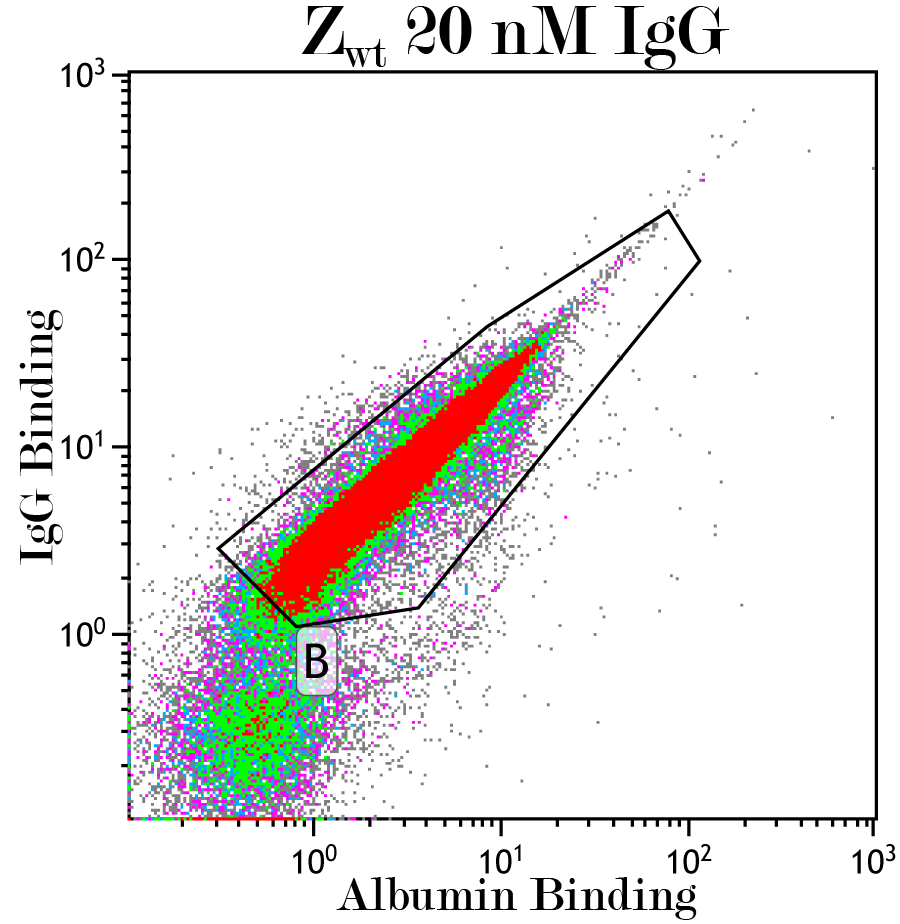
\includegraphics[width=\linewidth]{images/flow_20_wt.png}
			\label{flow_41}
		\end{subfigure}
		\begin{subfigure}{0.45\linewidth}
			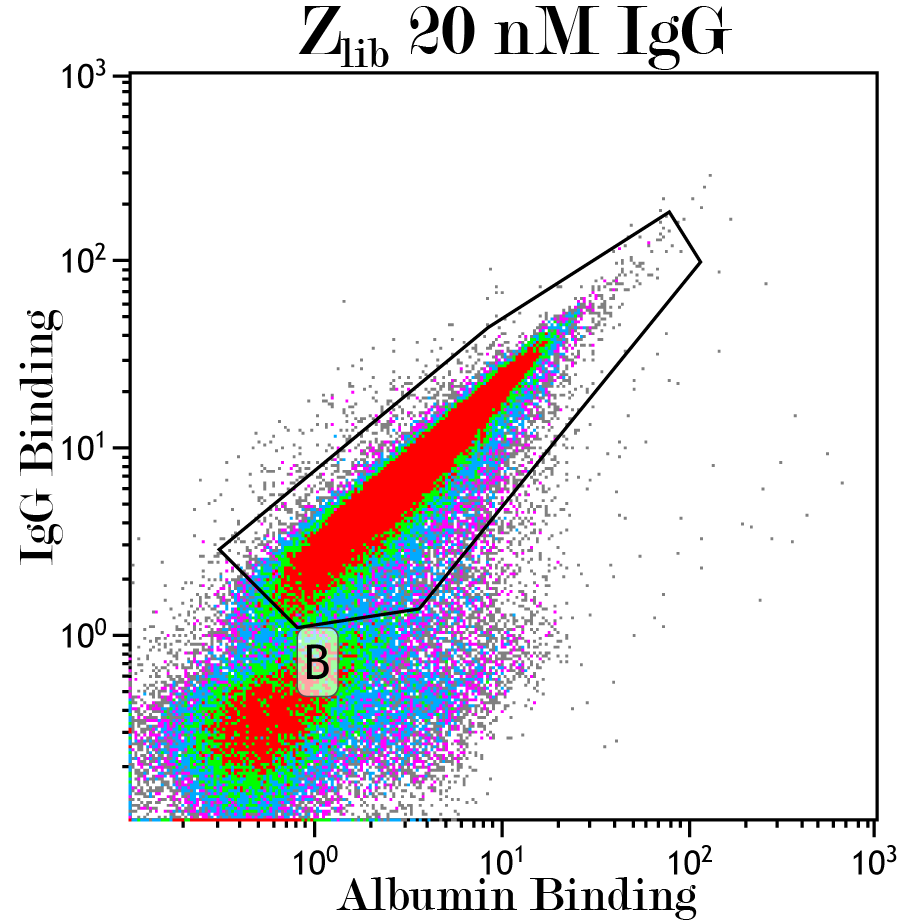
\includegraphics[width=\linewidth]{images/flow_20_lib.png}
			\label{flow_42}
		\end{subfigure}
	
		\begin{subfigure}{0.45\linewidth}
			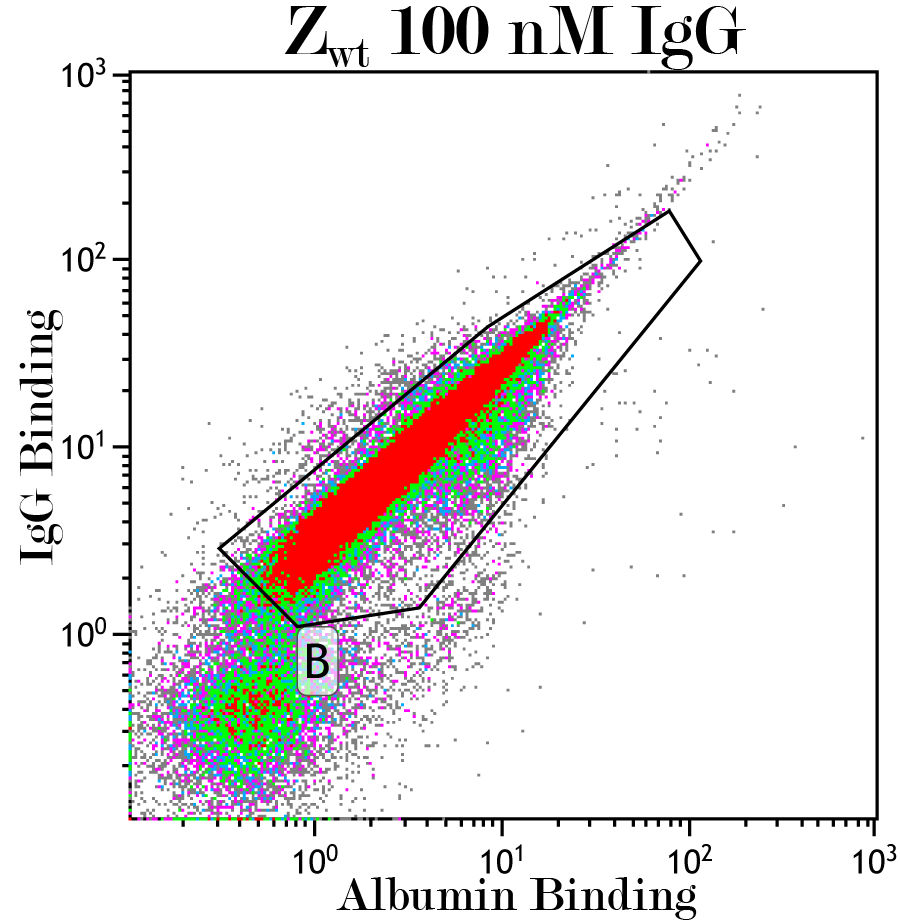
\includegraphics[width=\linewidth]{images/flow_100_wt.png}
			\label{flow_51}
		\end{subfigure}
		\begin{subfigure}{0.45\linewidth}
			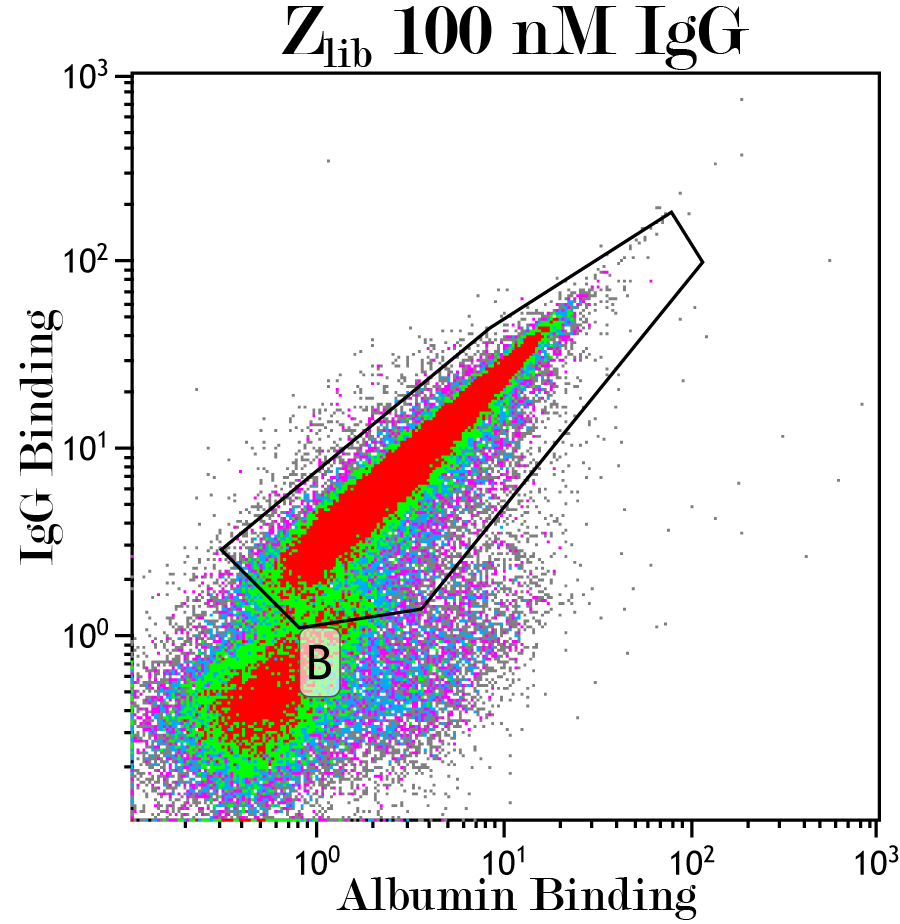
\includegraphics[width=\linewidth]{images/flow_100_lib.png}
			\label{flow_52}
		\end{subfigure}
		
		\centering
		\begin{subfigure}{0.45\linewidth}
			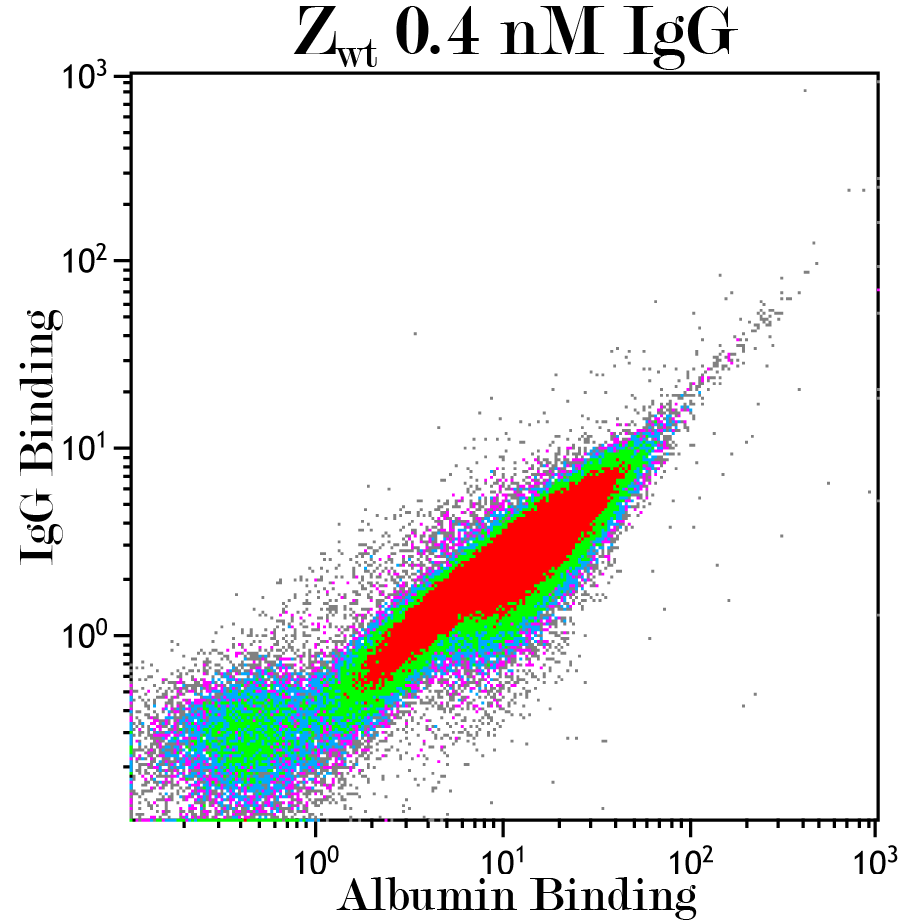
\includegraphics[width=\linewidth]{images/flow_04_wt.png}
			\label{flow_11}
		\end{subfigure}
		\begin{subfigure}{0.45\linewidth}
			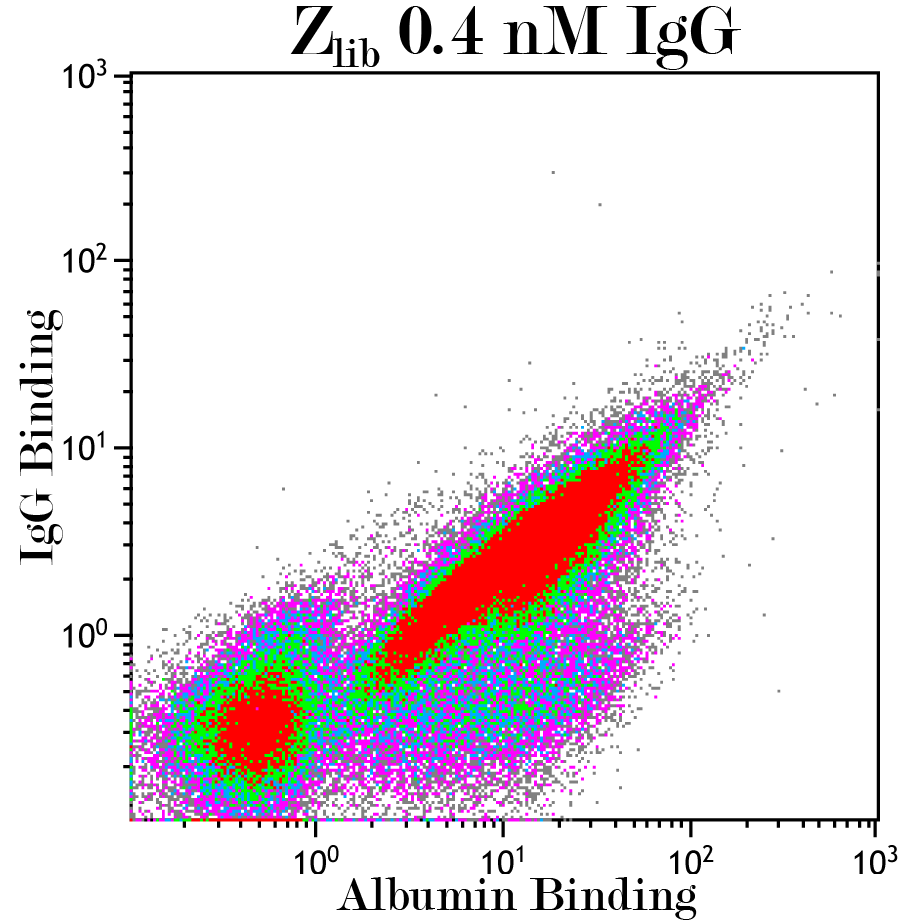
\includegraphics[width=\linewidth]{images/flow_04_lib.png}
			\label{flow_12}
			
		\end{subfigure}\hspace{15mm}
		\begin{subfigure}{0.45\linewidth}
			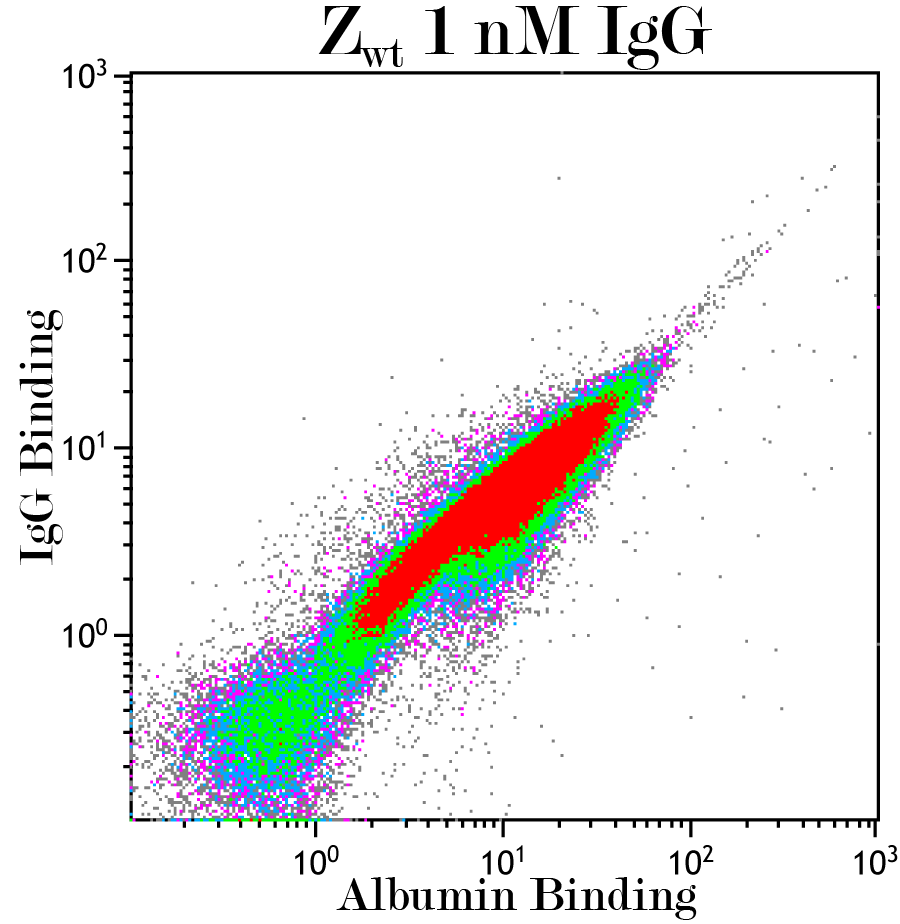
\includegraphics[width=\linewidth]{images/flow_1_wt.png}
			\label{flow_21}
		\end{subfigure}
		\begin{subfigure}{0.45\linewidth}
			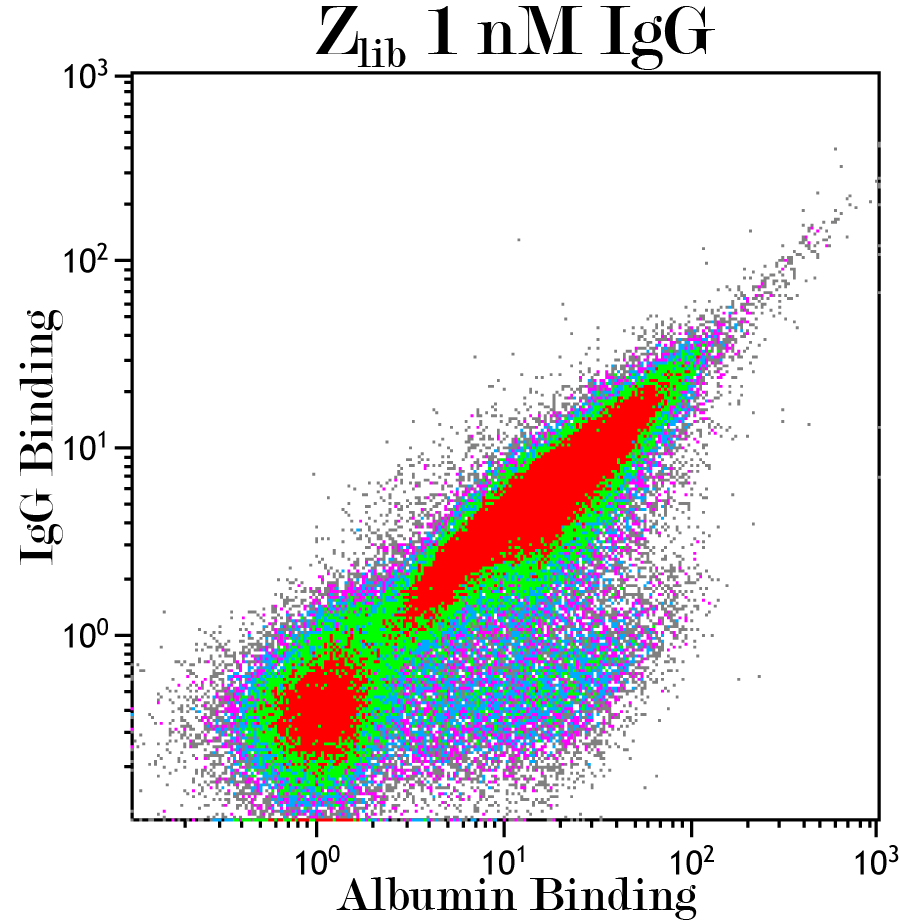
\includegraphics[width=\linewidth]{images/flow_1_lib.png}
			\label{flow_22}
		\end{subfigure}
	
		\begin{subfigure}{0.45\linewidth}
			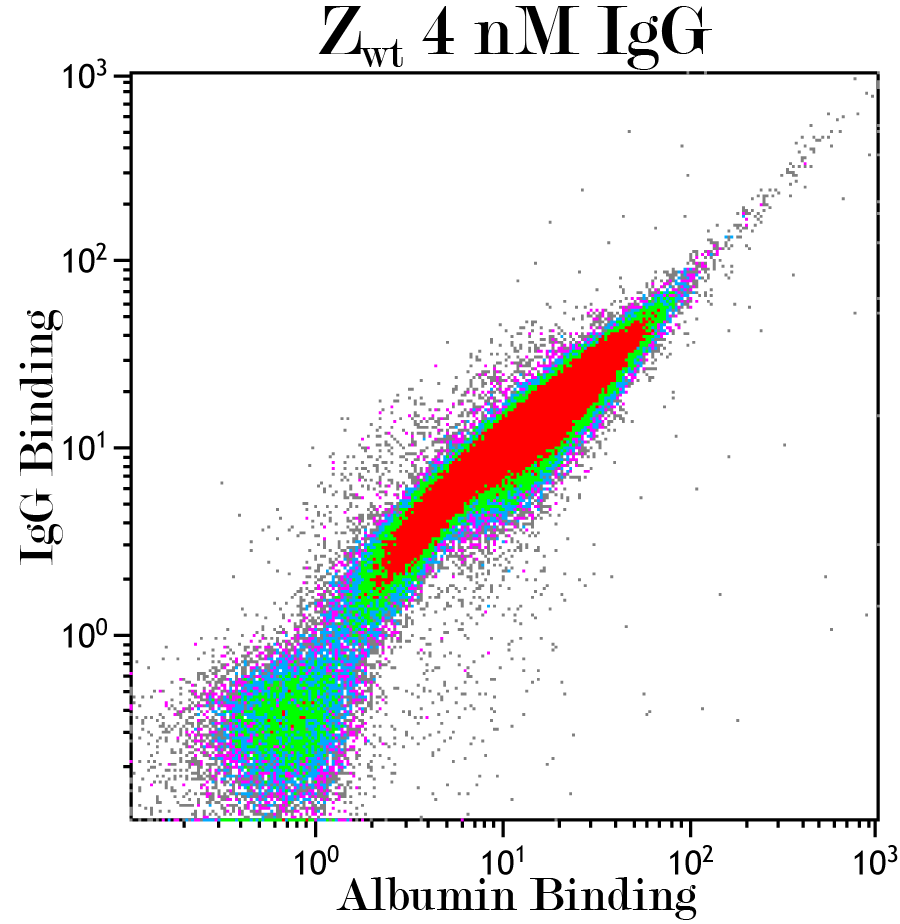
\includegraphics[width=\linewidth]{images/flow_4_wt.png}
			\label{flow_31}
		\end{subfigure}
		\begin{subfigure}{0.45\linewidth}
			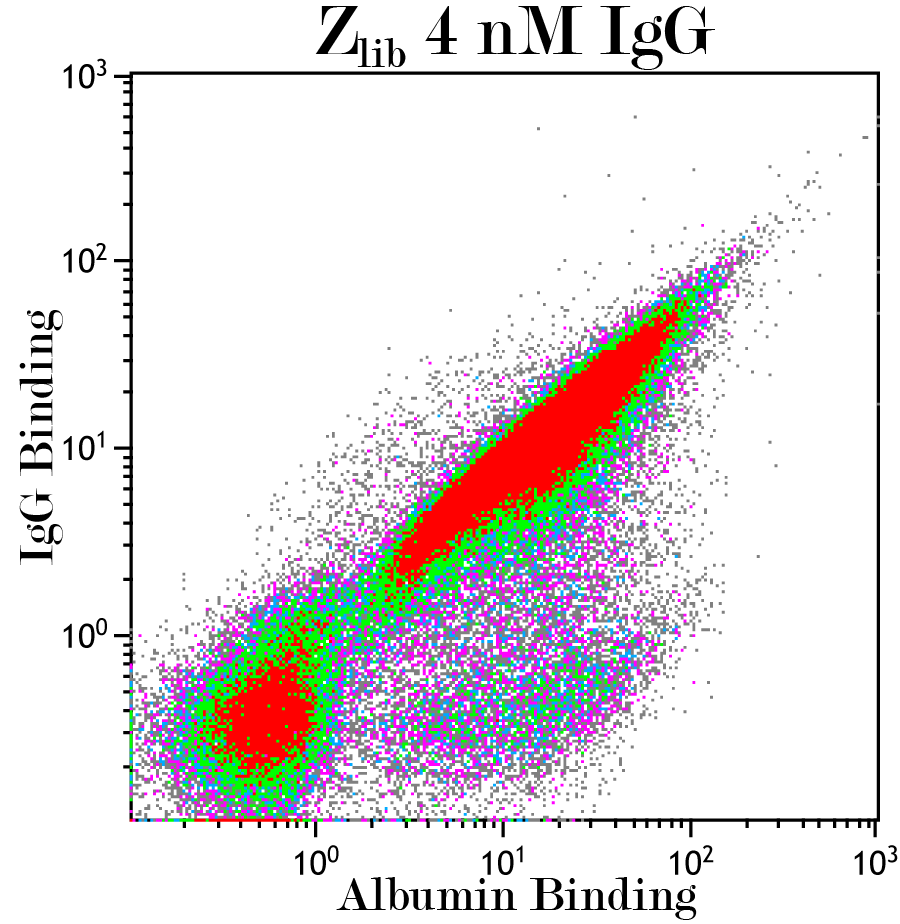
\includegraphics[width=\linewidth]{images/flow_4_lib.png}
			\label{flow_32}
		\end{subfigure}
	\caption{\textit{S.carnosus} cells with the wild type protein (left column) and library (right column) analyzed with flow cytometry.}
	\label{flow}
	\end{figure}
	
	In figure \ref{overlap} the results for the mutated plasmid and the wild type have been laid on top of each other to show the differences in affinity, the mutated plasmids are shown in red and the wild type in blue. This pictures clearly shows that the wild type have an overall higher affinity.
	
	\begin{figure}[H]
		\centering
		\begin{subfigure}{0.6\linewidth}
			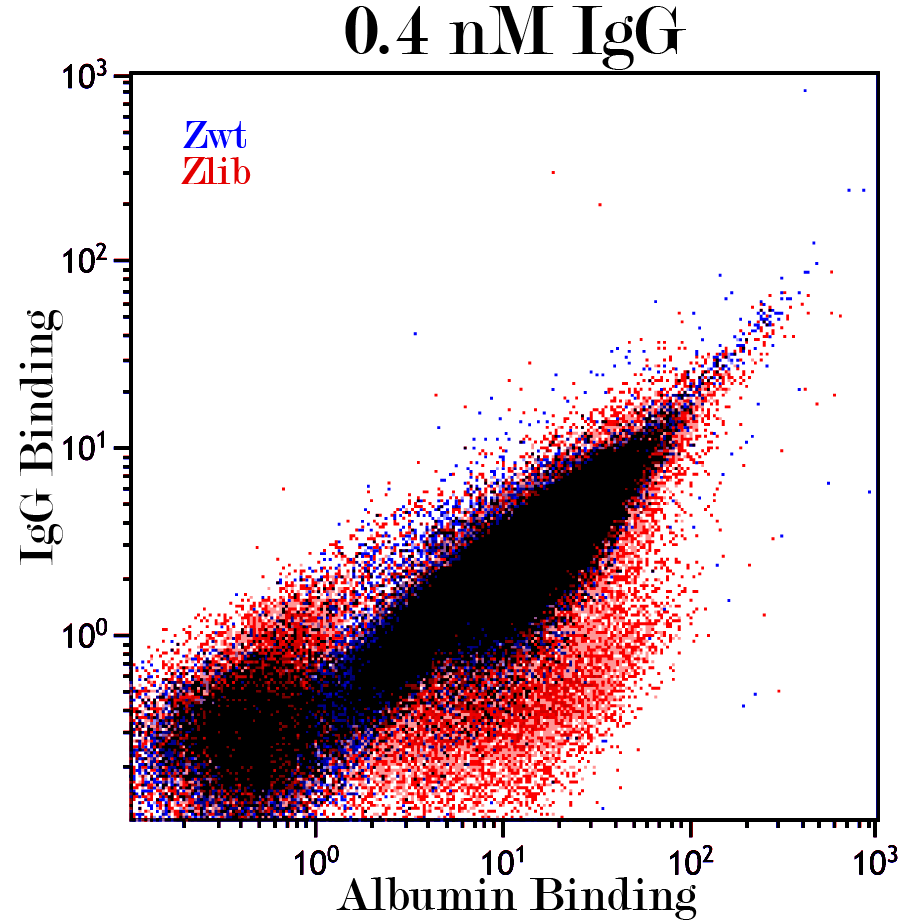
\includegraphics[width=\linewidth]{images/overlap_04.png}
		\end{subfigure}
		
		\begin{subfigure}{0.6\linewidth}
			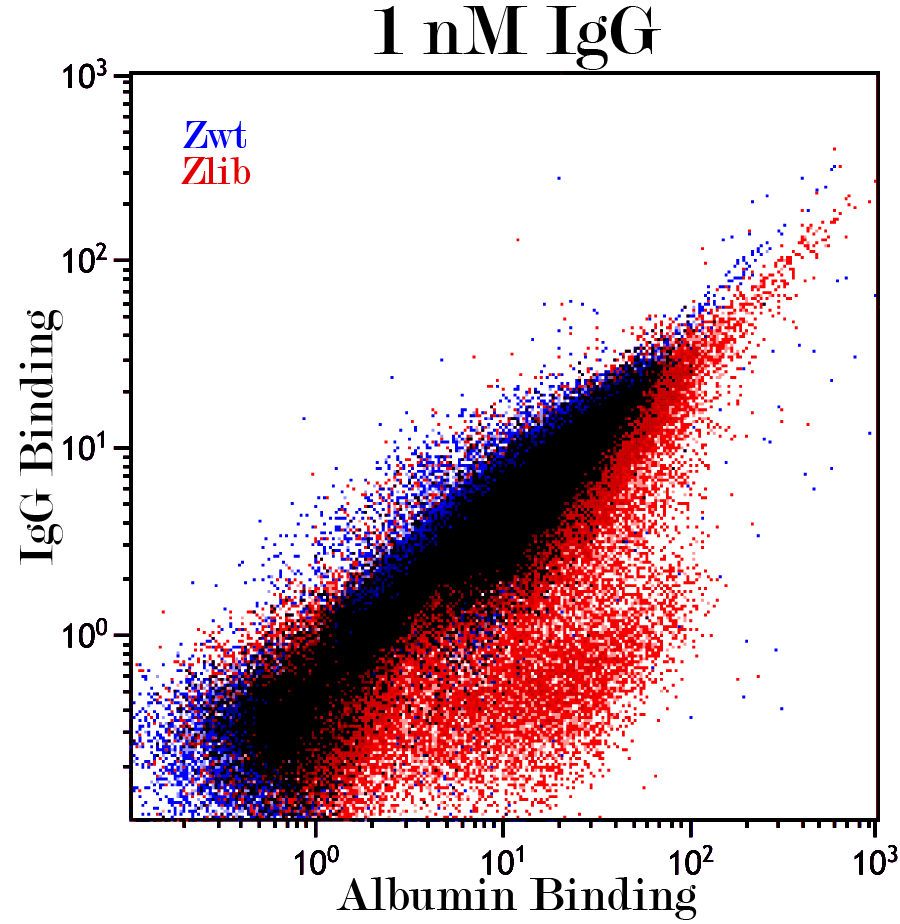
\includegraphics[width=\linewidth]{images/overlap_1.png}
		\end{subfigure}
	
		\begin{subfigure}{0.6\linewidth}
			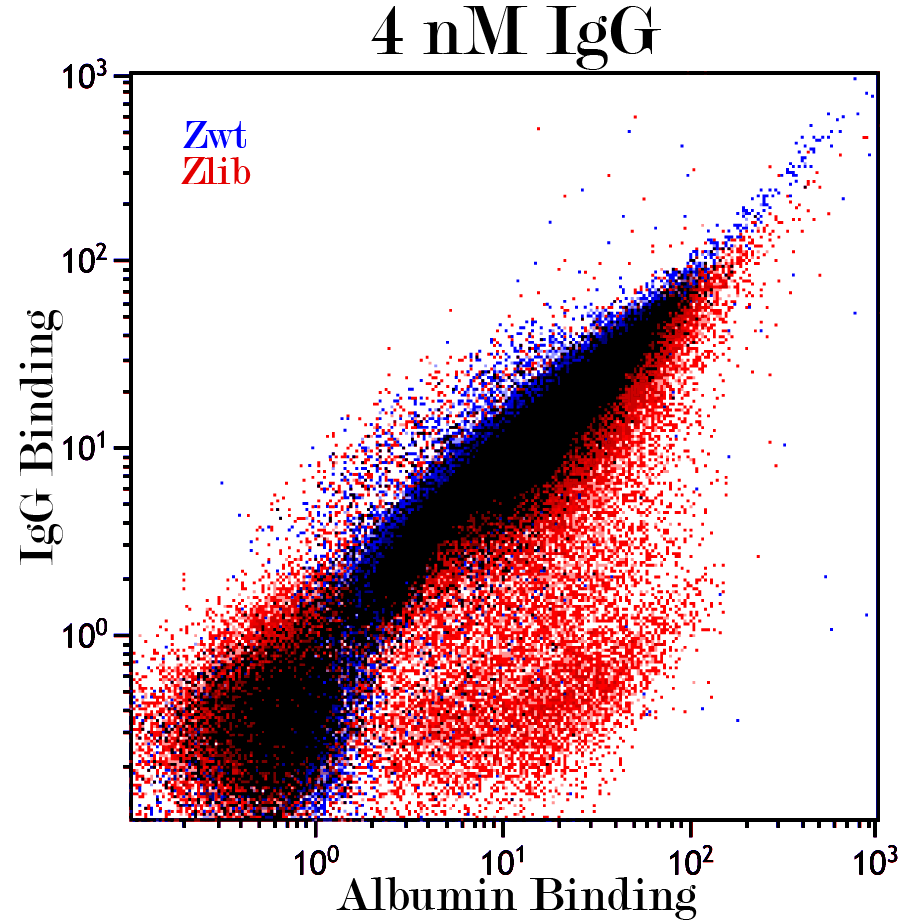
\includegraphics[width=\linewidth]{images/overlap_4.png}
		\end{subfigure}
		
		\caption{The density dot plots from the flow cytometry analysis of the \textit{S.carnosus} cells with the library and wild type overlayed. The cells with the library proteins are represented in red and the cells with the wild type protein are represented in blue. The y-axis is the IgG binding signal and the x-axis is the surface expression level.}
		\label{overlap}
	\end{figure}

	After having performed flow cytometry and found concentrations that worked, a FACS was performed to sort the cells based on affinity. The sorting was based on three gates dividing the cells into high, medium and low affinity. The high gate was used for two different samples with concentrations 0.4 and 10 nM. As seen in the pictures most of the cells are in the gate for high affinity.
	
	\begin{figure}[H]
		\centering
		\label{gate}
		\begin{subfigure}{0.8\linewidth}
			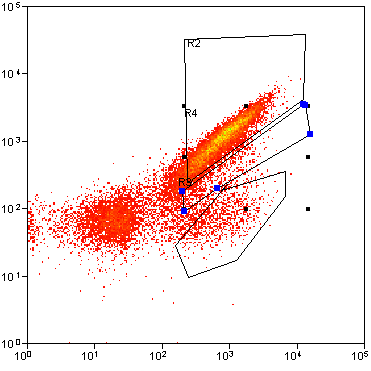
\includegraphics[width=\linewidth]{images/gate_3.png}
			\caption{10 nM IgG.}
		\end{subfigure}
		
		\begin{subfigure}{0.8\linewidth}
			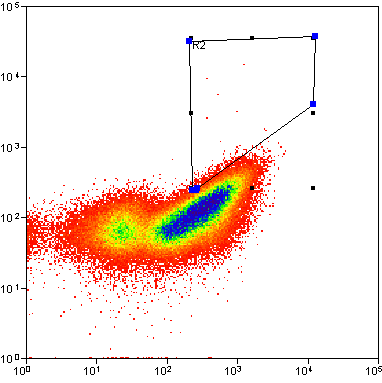
\includegraphics[width=\linewidth]{images/gate_1.png}
			\caption{0.4 nM IgG.}
		\end{subfigure}
		\caption{Density dot plot of the \textit{S.carnosus} cells with the library proteins analyzed and sorted into gates with flow cytometry. The y-axis is the IgG binding signal and the x-axis is the surface expression level.}
	\end{figure}

	\subsection{Sequence analysis}
	The final output of the script was the names of the sequencing wells, the position of substitution, the corresponding aa of the wild type and finally the corresponding aa of the variant, all arranged in columns and sorted by ascending position.
	
	This data can be found in appendix \ref{seqana}.
	
	Comments denoting discrepancies (if any), the full sequencing results, the aligned sequences and their corresponding aa sequences can also be found in the full results, which are not disclosed in this report for spacing reasons.
	
	\section{Discussion}
	The interpretation of the result is based on the gates from the plot diagrams in the FACS analysis. Sorting was performed and then 96 samples from each of the four gates were collected. From these sequenced samples, we have detected what specific mutations were present in each of the four groups. Data regarding all four gates is found in appendix \ref{seqana}.
	
	When comparing the flow cytometry results from the wild type protein to the library, no definite  conclusion can be drawn. The only definite conclusion is, when altering the protein many variants have got a lower affinity than the wild type protein. There are some library proteins that display a similar affinity as the wild type but not any that display a clearly higher affinity. It can be debated whether strains with higher affinities than wild type are present, and subsequent flow cytometry with pure strains of selected mutants could be used to determine relative affinity of a specific mutant. This could be investigated in a directed evolution experiment where subsequent FACS and growth sorts the library with regards to high binders.
	
	Conclusions that can be drawn from the data available from one cell sorting are based on the DNA sequences obtained from sequencing. Information about relative mutation frequency of different amino acid positions can be determined. The observed mutation frequency of a position in a affinity category relates to the effect said mutation has on the binding affinity. This is presented in figure \ref{freqana}. 
	
\end{multicols}
	\begin{figure}[H]
		\centering
		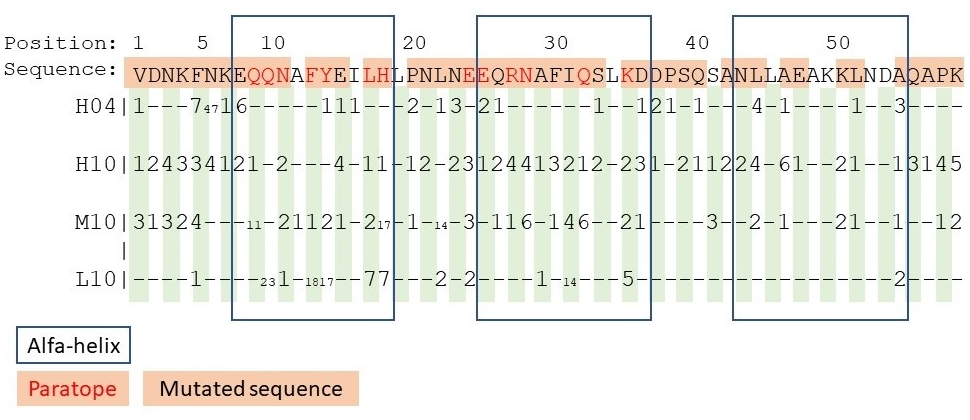
\includegraphics[width=\linewidth]{images/freqana_cut.jpg}
		\caption{The numbers represent the numbers of mutations per position in the different gates (H04, H10, M10 and L10). The paratope is represented in red and the mutated sequence is represented with orange. The alpha-helix is marked with black squares.}
		\label{freqana}
	\end{figure}
\begin{multicols}{2}	
	
	Position 10, 13, 14 och 31 were mutated in more than 75\% in total of the 96 cells taken from the gate with low affinity, at 10 nM IgG (L10). These positions are all located in the A and B alpha helix of the Z-domain. Position 10, 13 and 14 are part of the 13 positions initially suggested for mutation, and can be assumed to be amino acids displayed on the part of the surface that interacts with IgG and are therefore significant to affinity.
	
	Position 6 was mutated in almost 50\% of the cells with high affinity at 0.4nM IgG (H04), implying either great importance of the amino acid in that position, or no importance at all. A possible explanation for the high mutation frequency in position 6 could be that the amino acid asparagine is no good for the binding to IgG thus a mutation to any other amino acid is an advantage. As the high affinity binders had a similar affinity to Zwt, it can be assumed that the affinity is no better than Zwt. The mutation at position 6 presumably gives the same binding to IgG as the wild type and carries little importance. This is supported by the sequences (see appendix \ref{seqana}) which have mutations to 14 of the 20 different amino acids possible, and the fact that it is located outside any alpha helix.
	
	Position 9, 18 and 22 were highly mutated in the region of low affinity binders, but not non-binding to IgG at 10 nM IgG (M10). These positions were mutated to many different amino acids, which presumably affected and lowered the binding affinity. Two of these positions are located in alpha helix A, and included in the 13 positions of interest. It can be assumed that these positions are important for binding to IgG, but not essential as many different amino acids can be substituted and still provide affinity.
	
	The exploratory nature of this project offered an opportunity to explore all results and what information they could provide and not just be focused on one specific outcome. Since the affinity between IgG and Protein A already are used in the industry, there is interest in developing an improved affinity. The result from this project can therefore be used as a stepping stone to start exploring that possibility, even though this project was unable to do so. The project has the potential to identify single-point mutations and give useful information for future designing of saturation libraries. 
	
	The investigative nature of the project could also have been a threat to the project as there was no certainty as to whether or what result would be obtained. The time constraints on the project was also a factor in the results. If more time had been available more thorough investigations could have been made with a larger sample size, giving the possibility to alter the experiments to see if the results could be improved. Another possibility is investigating the folding and affinity of the protein \textit{in silico} and compare to the \textit{in vivo} results.
	
	Nowadays, the Z-domain is used in medical and biotechnological applications. Some of these applications and processes would be improved and made more efficient by a better bond, thereby benefiting from the results obtained by the project. An example of an application that can benefit from a higher affinity is the development of drugs with the use on antibodies, the application is based on a process where the Z domain can be used to immobilize or extract antibodies without affecting their active site. A better binding of the Z domain could here result in a higher yield of antibodies. 
	
	The pharmaceutical industry has a large turnover and a high economical yield on development. In the end it is possible to reduce the cost of pharmaceuticals. This can affect the world on a global scale, as drugs can be developed more easily, and become cheaper, making them more accessible and more able for society to benefit from. Higher yields in production stages also contribute to less wastage and lower emissions to the environment, or required resources in waste treatment. By doing experiments like this and continuing to explore possibilities for increased affinity, ultimately information obtained from such experiments could affect the problems described here.
	
	The optimal consequence of this project would be to influence humans and society in a positive way, giving people a healthier and higher quality of life. The experiment could also provide information beneficial for the environment, if more protein and antibody-based drugs were to be used. Today, most drugs available on the market are chemical-based \cite{noauthor_ifpma_nodate}, they can be difficult to break down when the molecules leave the body \cite{noauthor_pharmaceuticals_nodate}. In many cases, these chemicals have a negative impact on the environment, water quality and ecosystems. Protein-based drugs are developed based on protein found naturally in the body, IgG, this makes them easier to break down.

	\end{multicols}
	\newpage
	\bibliography{kex_sources}
	\bibliographystyle{vancouver}
	
	\newpage
	\appendix
	\section{Library}
	\label{lib_seq}
	Wild type aa sequence:
	\\KFTSQASDKKPTPRSAQDPLEVDNKFNKEQQNAFYEILHLPNLNEEQRNAFIQSLKDDP
	\\SQSANLLAEAKKLNDAQAPKVDLQACKLLDALAKAKADALKEFNKYGVSDYYKNLINN
	
	Length:\\117
	
	Substituted positions:\\22-32, 34-36, 38-39, 41-54, 56-61, 63-65, 67-68, 71-72
	
	Total number of substituted positions:\\48
	\newpage
	\section{Plasmid pSCCZ1 composition}
	\label{plasmid_map}

	\begin{figure}[H]
		\centering
		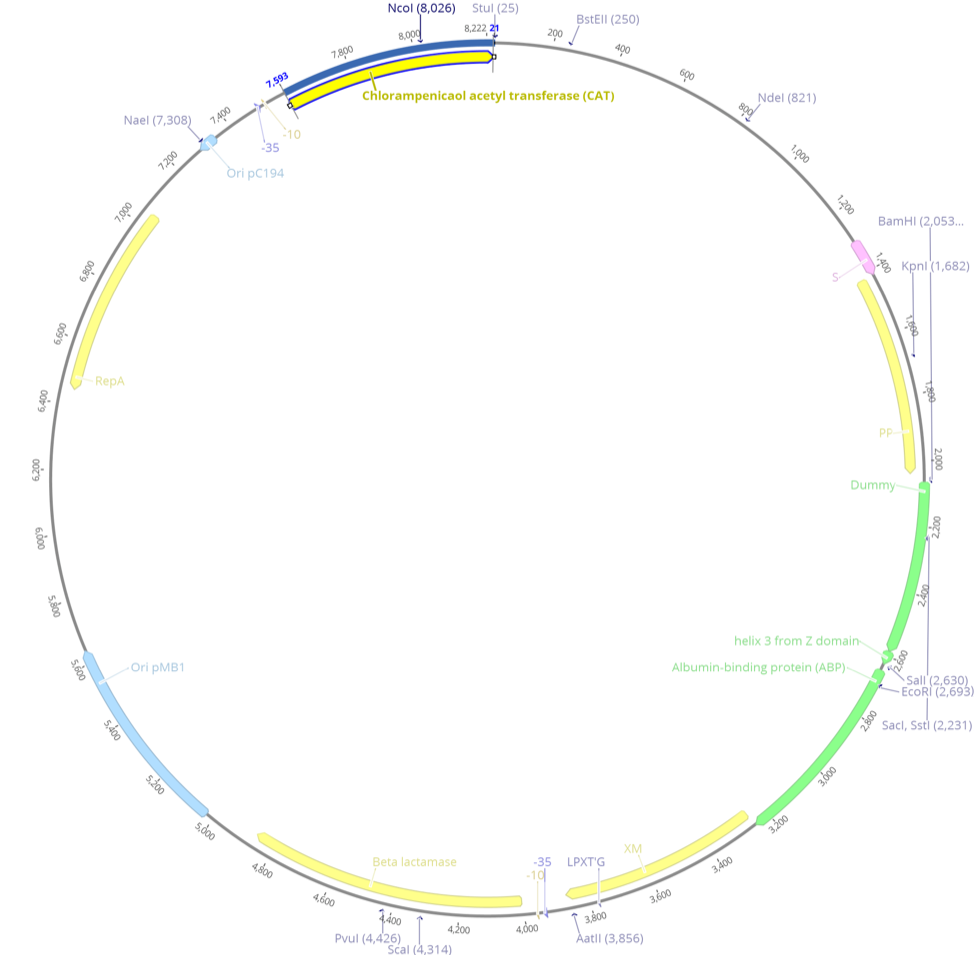
\includegraphics[width=0.8\linewidth]{images/dummy.png}
		\caption{Circular map showing the components of the plasmid pSCZ1.}
		\label{dummy}
	\end{figure}

	\section{Primer sequences}
	\label{primer_seq}
	
	\begin{table}[h!]
		\begin{center}
			\caption{Primers used for amplification of variants and plasmid for assembly.}
			
			\begin{tabular}{l|l} %alignments. left, automagic, r. there is also c for center
				\toprule %here
				\textbf{Denotation} & \textbf{Sequence} \\
				\midrule %here
				Plasmid forward & caggcatgcaagcttctagatgctc \\
				Plasmid reverse & tcctgcgcagatcttggtgttg \\
				Insert forward & agatctgcgcaggatcccct \\
				Insert reverse & aagcttgcatgcctgcaggtc \\
				SAPA23 & ? \\
				SAPA24 & ? \\
				\bottomrule %and here
				
			\end{tabular}
		\end{center}
	\end{table}

	\newpage
	\section{Calculation of library coverage}
	\label{calc}
	Let n be the number of variants 912 and N the number of transformed colonies 25146.
	\subsection{Calculation using standard fractional probabilities}
	The calculation uses the following assumptions:
	\begin{itemize}
		\item All variants are present at equal concentrations in the reaction mixture
		\item All variants are equally likely of being transformed
		\item All transformed variants are equally likely of growing
		\item The odds of encountering a particular variant is independent of the number of times that same variant has already been encountered
	\end{itemize}
	
	Hence, the probability of encountering a particular variant in one colony is
	\begin{equation}
	\frac{1}{n}
	\end{equation}
	the probability of not encountering a particular variant in one colony is
	\begin{equation}
	1-\frac{1}{n}
	\end{equation}
	the probability of not encountering a particular variant in at least one of all colonies is
	\begin{equation}
	(1-\frac{1}{n})^N
	\end{equation}
	the probability of encountering a particular variant in at least one of all colonies is
	\begin{equation}
	1-(1-\frac{1}{n})^N
	\end{equation}
	the probability p of encountering all particular variants in at least one of all colonies is
	\begin{equation}
	p = (1-(1-\frac{1}{n})^N)^n
	\end{equation}
	corresponding to a probability of 99.9999991\%.
	
	\subsection{Calculation using negative exponential distribution formula}
	
	\begin{equation}
	p = 1-e^{-\frac{N}{n}} \approx 1
	\end{equation}
	
	\newpage
	\section{Matlab script for sequence analysis}
	\label{script}
	\begin{lstlisting}[language=Matlab]
	%group = 'L';
	
	groupvector = cell(4,1);
	groupvector{1} = 'H04';
	groupvector{2} = 'H10';
	groupvector{3} = 'M';
	groupvector{4} = 'L';
	
	for groupcounter = 1:4
	group = groupvector{groupcounter};
	
	%Generate file names
	Alphabet = 'ABCDEFGHIJKLMNOPQRSTUVWXYZ';
	
	filenames_letters = num2str(zeros(96,1));
	filenames_numbers = zeros(96,1);
	letter = 1;
	for i = 1:12:96
	filenames_letters(i:i+11) = Alphabet(letter);
	letter = letter+1;
	for j = 0:11
	filenames_numbers(i+j) = j+1;
	end
	end
	filenames_numbers = num2str(filenames_numbers);
	
	for i = 1:96
	if str2num(filenames_numbers(i,:)) < 10
	filenames_numbers(i,:) = ['0' filenames_numbers(i,2)];
	end
	end
	
	filenames = cellstr(num2str(zeros(96,1)));
	wellnames = filenames;
	c = ['_', group ,'_SAPA-23.csv'];
	cID = ['_', group ,'_SAPA-23'];
	
	for i = 1:length(filenames)
	plateID(i) = {[filenames_letters(i) filenames_numbers(i,:)]}';
	filenames(i) = {[[filenames_letters(i) filenames_numbers(i,:)], c]};
	wellnames(i) = {[[filenames_letters(i) filenames_numbers(i,:)], cID]};
	end
	
	% Rip sequences
	seq_long = cell(96,1);
	foldername = [group, '_sapa23_csv\'];
	for i = 1:96
	[num, txt] = xlsread([foldername, filenames{i}], 'A2:A2');
	seq_long(i) = txt;
	end
	
	% Define sequences
	seq_plasmid = [[See other appendices]];
	aa_plasmid = DNAtranslator(seq_plasmid(1:end-2));
	aa_wt = [[See other appendices]];
	seq_wt = seq_plasmid(668*3-2 : 668*3-2+117*3-1);
	aa_comp = [[See other appendices]];
	seq_comp = seq_plasmid(689*3-2 : 689*3-2+length(aa_comp)*3-1);
	
	preZ = seq_plasmid(2064-19:2064);
	postZ = seq_plasmid(2065+length(seq_comp):2065+length(seq_comp)+19);
	
	% Trim and classify
	seq = seq_long;
	comment = cell(96,1);
	error_fail = 'Sequencing failed';
	error_short = 'Sequence too short to align successfully';
	error_N = 'Z-domain contains undetermined bases. Check reverse sequence';
	error_indel = 'Sequence contains insertions or deletions';
	error_wt = 'Sequence is wild-type';
	error_align = 'Alignment failed';
	
	for i = 1:96
	% Cut-out comp. seq.
	if length(seq_long{i}) >= 174+2*20
	Zstart = strfind(seq_long{i}, preZ) + length(preZ);
	Zend = strfind(seq_long{i}, postZ) -1;
	seq{i} = seq_long{i}(Zstart:Zend);
	elseif length(seq_long{i}) == 5 && mean(seq_long{i} == 'NNNNN') == 1
	comment{i} = error_fail;
	seq{i} = seq_long{i};
	elseif isempty(comment{i}) == 1 && length(seq_long{i}) < 174+2*20
	comment{i} = error_short;
	seq{i} = seq_long{i};
	else
	comment{i} = error_align;
	seq{i} = seq_long{i};
	end
	% Is comp. seq. longer/shorter/wt?
	if isempty(comment{i}) == 1 && length(seq{i}) ~= length(seq_comp)
	comment{i} = error_indel;
	elseif isempty(comment{i}) == 1 && length(seq{i}) == length(seq_comp)
	if seq{i} == seq_comp
	comment{i} = error_wt;
	end
	end
	% Does comp. seq. contain bases other than ACTG?
	if isempty(comment{i}) == 1 && length(seq_long{i}) >= 174 ...
	&& length(strfind(seq{i}, 'A')) + length(strfind(seq{i}, 'T')) ...
	+ length(strfind(seq{i}, 'C')) + length(strfind(seq{i}, 'G')) < length(seq{i})
	comment{i} = error_N;
	elseif isempty(comment{i}) ~= 1 && length(seq_long{i}) >= 174 && ...
	length(strfind(seq{i}, 'A')) + length(strfind(seq{i}, 'T')) ...
	+ length(strfind(seq{i}, 'C')) + length(strfind(seq{i}, 'G')) < length(seq{i})
	comment{i} = [comment{i},' & ', error_N];
	end
	end
	
	% Translate sequences
	aa = cell(96,1);
	counter = 0;
	for i = 1:96
	counter = counter +1;
	if isempty(comment{i}) == 1
	aa{i} = DNAtranslator(seq{i});
	else
	aa{i} = '-';
	end
	end
	
	% Compare to wt seq
	subsIndex = cell(96,1);
	subsFrom = subsIndex;
	subsTo = subsIndex;
	
	for i = 1:96
	if isempty(comment{i}) == 1
	subsIndex{i} = find((aa{i} == aa_comp) == 0);
	subsFrom(i,1) = {aa_comp(subsIndex{i,1})};
	subsTo(i,1) = {aa{i}(subsIndex{i,1})};
	else
	subsFrom(i,1) = {'-'};
	subsTo(i,1) = {'-'};
	subsIndex{i,1} = '-';
	end
	end
	
	% Switch index to position
	position = cell(96,1);
	for i = 1:96
	if isnumeric(subsIndex{i}) == 1
	position{i} = subsIndex{i} + 21;
	else
	position{i} = subsIndex{i};
	end
	
	if length(position{i}) > 1
	position_merge = zeros(1,length(position{i}));
	for j = 1:length(position{i})
	position_merge(j) = position{i}(j);
	end
	position{i} = num2str(position_merge);
	comment{i} = 'Multiple substitutions';
	end
	end
	
	% Sort
	
	for i = 1:96
	if isnumeric(position{i}) == 1
	position_sort(i,1) = position{i};
	else
	position_sort(i,1) = 0;
	end
	end
	
	[sortVal, sortIndex] = sort(position_sort);
	
	output = cell(96,8);
	output(:,1) = wellnames(:,1);
	output(:,2) = comment(:,1);
	output(:,3) = seq_long(:,1);
	output(:,4) = seq(:,1);
	output(:,5) = aa(:,1);
	output(:,6) = position(:,1);
	output(:,7) = subsFrom(:,1);
	output(:,8) = subsTo(:,1);
	
	output_sorted = cell(96,8);
	
	for i = 1:96
	for j = 1:8
	output_sorted{i,j} = output{sortIndex(i),j};
	end    
	end
	
	headers = {'Well name', 'Comment', 'Full NT sequence' ...
	'Aligned NT sequence', 'Aligned AA sequence', 'AA position'...
	'From AA', 'To AA'};
	output_sorted
	
	xlswrite('results.xls', headers, group, 'A1:H1')
	xlswrite('results.xls', output_sorted, group, 'A2:H97')
	
	end
	\end{lstlisting}
	\newpage
	\section{aa substitutions}
	\label{seqana}
	\begin{multicols}{2}
	\begin{table}[H]
		\begin{center}
			\caption{High binders at IgG concentration 0.4 nm}
			{\Large \textbf{Wells 1-48}}
			\vspace{3mm}
			
			\pgfplotstabletypeset[
			multicolumn names, % allows to have multicolumn names
			col sep=comma, % the seperator in our .csv file
			display columns/0/.style={
				column name=Well name, % name of first column
				column type={c},string type},  % use siunitx for formatting
			display columns/1/.style={
				column name=AA position,
				column type={c},string type},
			display columns/2/.style={
				column name=From AA,
				column type={c},string type},		
			display columns/3/.style={
				column name=To AA,
				column type={c},string type},					
			every head row/.style={
				before row={\toprule}, % have a rule at top
				after row={
					\midrule} % rule under units
			},
			every last row/.style={after row=\bottomrule}, % rule at bottom
			]{h04a.csv} % filename/path to file
		\end{center}
	\end{table}
	
	\begin{table}[H]
		\begin{center}
			\vspace{7.8mm}
			{\Large \textbf{Wells 49-96}}
			\vspace{3mm}
			
			\pgfplotstabletypeset[
			multicolumn names, % allows to have multicolumn names
			col sep=comma, % the seperator in our .csv file
			display columns/0/.style={
				column name=Well name, % name of first column
				column type={c},string type},  % use siunitx for formatting
			display columns/1/.style={
				column name=AA position,
				column type={c},string type},
			display columns/2/.style={
				column name=From AA,
				column type={c},string type},		
			display columns/3/.style={
				column name=To AA,
				column type={c},string type},					
			every head row/.style={
				before row={\toprule}, % have a rule at top
				after row={
					\midrule} % rule under units
			},
			every last row/.style={after row=\bottomrule}, % rule at bottom
			]{h04b.csv} % filename/path to file
		\end{center}
	\end{table}
	\end{multicols}

	\newpage
	\begin{multicols}{2}
		\begin{table}[H]
			\begin{center}
				\caption{High binders at IgG concentration 10 nm}
				{\Large \textbf{Wells 1-48}}
				\vspace{3mm}
				
				\pgfplotstabletypeset[
				multicolumn names, % allows to have multicolumn names
				col sep=comma, % the seperator in our .csv file
				display columns/0/.style={
					column name=Well name, % name of first column
					column type={c},string type},  % use siunitx for formatting
				display columns/1/.style={
					column name=AA position,
					column type={c},string type},
				display columns/2/.style={
					column name=From AA,
					column type={c},string type},		
				display columns/3/.style={
					column name=To AA,
					column type={c},string type},					
				every head row/.style={
					before row={\toprule}, % have a rule at top
					after row={
						\midrule} % rule under units
				},
				every last row/.style={after row=\bottomrule}, % rule at bottom
				]{h10a.csv} % filename/path to file
			\end{center}
		\end{table}
		
		\begin{table}[H]
			\begin{center}
				\vspace{7.8mm}
				{\Large \textbf{Wells 49-96}}
				\vspace{3mm}
				
				\pgfplotstabletypeset[
				multicolumn names, % allows to have multicolumn names
				col sep=comma, % the seperator in our .csv file
				display columns/0/.style={
					column name=Well name, % name of first column
					column type={c},string type},  % use siunitx for formatting
				display columns/1/.style={
					column name=AA position,
					column type={c},string type},
				display columns/2/.style={
					column name=From AA,
					column type={c},string type},		
				display columns/3/.style={
					column name=To AA,
					column type={c},string type},					
				every head row/.style={
					before row={\toprule}, % have a rule at top
					after row={
						\midrule} % rule under units
				},
				every last row/.style={after row=\bottomrule}, % rule at bottom
				]{h10b.csv} % filename/path to file
			\end{center}
		\end{table}
	\end{multicols}

	\newpage
	\begin{multicols}{2}
		\begin{table}[H]
			\begin{center}
				\caption{Medium binders at IgG concentration 10 nm}
				{\Large \textbf{Wells 1-48}}
				\vspace{3mm}
				
				\pgfplotstabletypeset[
				multicolumn names, % allows to have multicolumn names
				col sep=comma, % the seperator in our .csv file
				display columns/0/.style={
					column name=Well name, % name of first column
					column type={c},string type},  % use siunitx for formatting
				display columns/1/.style={
					column name=AA position,
					column type={c},string type},
				display columns/2/.style={
					column name=From AA,
					column type={c},string type},		
				display columns/3/.style={
					column name=To AA,
					column type={c},string type},					
				every head row/.style={
					before row={\toprule}, % have a rule at top
					after row={
						\midrule} % rule under units
				},
				every last row/.style={after row=\bottomrule}, % rule at bottom
				]{ma.csv} % filename/path to file
			\end{center}
		\end{table}
		
		\begin{table}[H]
			\begin{center}
				\vspace{7.8mm}
				{\Large \textbf{Wells 49-96}}
				\vspace{3mm}
				
				\pgfplotstabletypeset[
				multicolumn names, % allows to have multicolumn names
				col sep=comma, % the seperator in our .csv file
				display columns/0/.style={
					column name=Well name, % name of first column
					column type={c},string type},  % use siunitx for formatting
				display columns/1/.style={
					column name=AA position,
					column type={c},string type},
				display columns/2/.style={
					column name=From AA,
					column type={c},string type},		
				display columns/3/.style={
					column name=To AA,
					column type={c},string type},					
				every head row/.style={
					before row={\toprule}, % have a rule at top
					after row={
						\midrule} % rule under units
				},
				every last row/.style={after row=\bottomrule}, % rule at bottom
				]{mb.csv} % filename/path to file
			\end{center}
		\end{table}
	\end{multicols}

	\newpage
	\begin{multicols}{2}
		\begin{table}[H]
			\begin{center}
				\caption{Low binders at IgG concentration 10 nm}
				{\Large \textbf{Wells 1-48}}
				\vspace{3mm}
				
				\pgfplotstabletypeset[
				multicolumn names, % allows to have multicolumn names
				col sep=comma, % the seperator in our .csv file
				display columns/0/.style={
					column name=Well name, % name of first column
					column type={c},string type},  % use siunitx for formatting
				display columns/1/.style={
					column name=AA position,
					column type={c},string type},
				display columns/2/.style={
					column name=From AA,
					column type={c},string type},		
				display columns/3/.style={
					column name=To AA,
					column type={c},string type},					
				every head row/.style={
					before row={\toprule}, % have a rule at top
					after row={
						\midrule} % rule under units
				},
				every last row/.style={after row=\bottomrule}, % rule at bottom
				]{la.csv} % filename/path to file
			\end{center}
		\end{table}
		
		\begin{table}[H]
			\begin{center}
				\vspace{7.8mm}
				{\Large \textbf{Wells 49-96}}
				\vspace{3mm}
				
				\pgfplotstabletypeset[
				multicolumn names, % allows to have multicolumn names
				col sep=comma, % the seperator in our .csv file
				display columns/0/.style={
					column name=Well name, % name of first column
					column type={c},string type},  % use siunitx for formatting
				display columns/1/.style={
					column name=AA position,
					column type={c},string type},
				display columns/2/.style={
					column name=From AA,
					column type={c},string type},		
				display columns/3/.style={
					column name=To AA,
					column type={c},string type},					
				every head row/.style={
					before row={\toprule}, % have a rule at top
					after row={
						\midrule} % rule under units
				},
				every last row/.style={after row=\bottomrule}, % rule at bottom
				]{lb.csv} % filename/path to file
			\end{center}
		\end{table}
	\end{multicols}
\end{document}